% Correcting the title chapter page
\fancypagestyle{plain}{%
    \fancyhf{}
    \fancyhead[RO,LE]{\bfseries \thepage}
    \fancyhead[CO]{\rightmark}
    \fancyhead[CE]{\leftmark}
    \renewcommand{\headrulewidth}{0.4pt}}

\chapter{Liejeve grupe}
\label{ch:lie}

\section{Kontinuirane grupe}


U prva tri poglavlja smo upoznali \emph{konačne grupe} kao skupove
konačnog broja elemenata na kojima je definirana binarna operacija (tablica množenja)
koja zadovoljava četiri aksioma (vidi definiciju \ref{def:grupa}). 
U fizici elemente grupe povezujemo
s transformacijama simetrije i pripadajući skup operatora transformacija
zovemo reprezentacija grupe. Pokazali smo da reprezentacije konačnih grupa
zadovoljavaju neka netrivijalna svojstva koja se onda odražavaju
i na netrivijalnim svojstvima fizikalnih objekata poput kristala.
No cijelim putem, a posebice u prošlom poglavlju, vidjeli smo da neke
od najvažnijih simetrija, poput rotacija i translacija prostora,
nisu konačne. Za razliku od kristala, prazan prostor ili električno
polje naboja u ishodištu su simetrični na rotaciju oko bilo koje
osi (kroz ishodište), kojih ima beskonačno, i za bilo koji kut, kojih
isto ima beskonačno. Dakle, odgovarajuća grupa će imati beskonačni
broj elemenata. Tako za nju nećemo moći napisati grupnu tablicu
množenja, a čini se problematično i to da smo se u dokazivanju
najvažnijih teorema teorije reprezentacija oslanjali na konačnost
grupe.

Srećom, uz tu komplikaciju svoje beskonačnosti, navedene grupe obično donose
i iskupljujuće svojstvo \emph{kontinuiranosti} koje nam onda dodatno
stavlja na raspolaganje moćne matematičke teorije infinitezimalnog računa,
tj. realne i kompleksne analize te diferencijalne geometrije i topologije.
Zahvaljujući tome matematička teorija kontinuiranih grupa je u nekim aspektima
čak i jednostavnija od teorije konačnih grupa\footnote{Najspektakularniji
    primjer je potpuna klasifikacija grupa koju je za kontinuirane
    grupe dovršio još E. Cartan i koja se često izlaže u jednom poglavlju
    čak i udžbenika za studente fizike, poput \cite{Jones:1998}, dok je
    klasifikacija konačnih grupa dovršena tek krajem 20. stoljeća i razbacana
je na tisuće stranica specijalizirane matematičke literature.}.


U nedostatku mogućnosti da pojedinačno navedemo sve elemente beskonačnih
grupa, za razmatranje istih uvodimo važan pojam \emph{grupnog prostora}
kojeg nazivamo i \emph{grupna mnogostrukost}.
Riječ je o prostoru čija je svaka točka pridružena jedinstvenom
elementu grupe.
Za konačne grupe \emph{grupni prostor} je naprosto skup točaka koji
nema neka dodatna svojstva povrh svojstava koji mu daju aksiomi grupe
(dakle, ne smatramo da su te točke elementi nekog pravca, ravnine
ili višedimenzionalnog prostora):

\centerline{\documentclass[border=3mm]{standalone}

\usepackage{tikz}

\begin{document}
	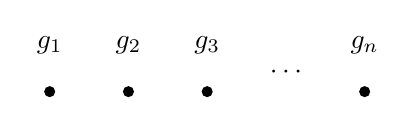
\begin{tikzpicture}
		\fill (0,0) circle (2pt) node[above,yshift=10pt] {$g_1$};
		\fill (1,0) circle (2pt) node[above,yshift=10pt] {$g_2$};
		\fill (2,0) circle (2pt) node[above,yshift=10pt] {$g_3$};
		\node at (3,0.25) {$\cdots$};
		\fill (4,0) circle (2pt) node[above,yshift=10pt] {$g_n$};
	\end{tikzpicture}
\end{document}}
%\centerline{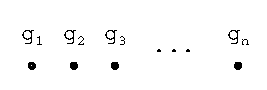
\includegraphics[scale=1.0]{pics/grupni_prostor.eps}}

S druge strane za \emph{kontinuirane beskonačne grupe} grupni prostor je
kontinuum točaka koji \emph{ima} dodatna matematička svojstva. 
Ovisno o razini općenitosti, prostori s takvim dodatnim svojstvima dolaze pod
nazivima \emph{topološki prostor} ili \emph{diferencijabilna mnogostrukost},
za čije je matematički korektno specificiranje potrebno uvesti
niz sofisticiranih matematičkih koncepata (vidi npr. 
\cite{Smolic:2024}). Za naše potrebe dovoljno je reći da su grupni
prostori lokalno slični prostoru $\mathbb{R}^n$,
tj. da ih je lokalno moguće parametrizirati $n$-torkom realnih\footnote{Matematičari
    poznaju i grupe čiji grupni prostor se parametrizira kompleksnim
    brojevima, no mi ovdje takve grupe nećemo sresti.}
brojeva. Najbolje je to razjasniti na primjerima.


Grupa $\{R(\unitn, \theta) \td \theta\in[0,2\pi)\}$ svih rotacija oko zadane osi
$\unitn$ ima kao grupnu mnogostrukost kružnicu jer točke na kružnici možemo parametrizirati
kao $(r\cos\theta, r\sin\theta)$ i tako uspostaviti bijektivno preslikavanje
između točaka kružnice i elemenata grupe. 
Ovdje je radijus $r$ nebitan, svaka kružnica je ekvivalentna kao
grupni prostor. Štoviše, ni oblik nije ključan pa bi i elipsa mogla poslužiti.
No kako se u računima oslanjamo na parametrizaciju grupe pomoću
kuta $\theta$ bit će računski najjednostavnije držati se kružnice.
Sa stanovišta teorije grupa, jedina bitna svojstva su kontinuiranost krivulje
koja odražava kontinuiranost grupe i \emph{topologija} kružnice tj. činjenica da 
kontinuiranim povećavanjem kuta rotacije do $2\pi$ dolazimo natrag do jediničnog
elementa, tj. rotacije za nula stupnjeva.
Upravo ta parametrizacija jednim realnim brojem $\theta$ je ono na što
se misli kad se kaže da je grupna mnogostrukost lokalno slična $\mathbb{R}^n$,
gdje je u ovom slučaju $n=1$.).
No sličnost nije globalna zbog različite topologije kružnice
i $\mathbb{R}^1$.

\centerline{\documentclass[border=3mm]{standalone}

\usepackage{tikz}
\usetikzlibrary{3d,arrows.meta}

\begin{document}
	\begin{tikzpicture}
		\begin{scope}
			\draw[very thick] (0,0) circle (2cm);
			\fill (0,2) circle (2pt) node[above]{$R(0)$};
			\fill (0,-2) circle (2pt) node[below]{$R(\pi)$};
		\end{scope}
		\begin{scope}[canvas is xz plane at y=0,xshift=6cm]
			\draw[very thick] (-2,-2) rectangle (2,2);
			\draw[-Triangle] (-1,1.5) -- (-1,-0.5) node[above]{$t_2$};
			\draw[-Triangle] (-1.5,1) -- (0,1) node[right]{$t_1$};
			\fill (0.7,-1) circle (2pt) node[right]{$(t_1,t_2)$};
		\end{scope}
	\end{tikzpicture}
\end{document}}
%\centerline{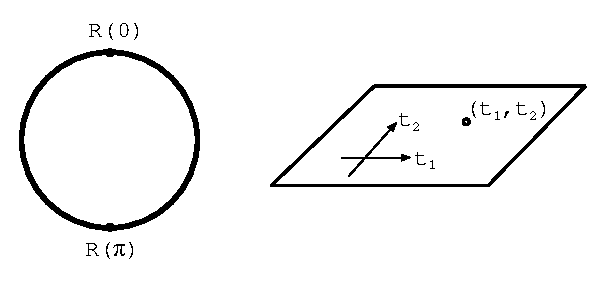
\includegraphics[scale=1.0]{pics/mnogostrukost.eps}}

Kao drugi primjer promotrimo grupu svih translacija u ravnini $\vec{x}\to\vec{x}+\vec{t}$,
dakle translacija za bilo koji vektor $\vec{t}=(t_1, t_2)$.
Ovdje je elemente grupe prirodno parametrizirati dvama
realnim brojevima $t_1, t_2 \in (-\infty, \infty)$ i očito je da je
 grupna mnogostrukost ravnina tj. $\mathbb{R}^2$. Ovdje naravno treba
 razlikovati ravninu koja je vektorski prostor čije vektore transformiraju
 elementi grupe
 (tj. strogo uzevši njene reprezentacije) i ravninu koja je grupni prostor za koji uopće
 nije nužno da ima svojstva vektorskog prostora.

Kako vidimo iz ova dva primjera, elemente kontinuiranih grupa identificiramo
s točkama $n$-dimenzionalne grupne mnogostrukosti koju
parametriziramo s $n$ realnih brojeva
  $(a_1, a_2, \ldots, a_n)$,
te onda govorimo o \emph{$n$-parametarskoj} ili \emph{$n$-dimenzionalnoj} grupi.
Zahvaljajući toj identifikaciji
elemente grupe ćemo označavati kao $g(a_1, a_2, \ldots, a_n)$, odnosno
skraćeno $g(a)$.

Promotrimo sada četiri aksioma grupe u svjetlu ove diskusije.
\begin{enumerate}
\item Zatvorenost: $g(c)=g(a)g(b) \in G$. Umjesto tablice množenja koja
    je definirala grupnu operaciju, sada nam treba funkcija, tzv.
    funkcija kompozicije
    \[\phi: G\times G \to G \quad  \text{tako da je} \quad c=\phi(a,b) \]
    (Npr. za rotacije oko date osi imamo $R(\theta) = R(\theta_1) R(\theta_2)$
    gdje je funkcija kompozicije  $\theta = \phi(\theta_1, \theta_2) =
    (\theta_1 + \theta_2)\, \mathrm{mod}\, 2\pi$ .) U svjetlu identifikacije
    grupe i njenog grupnog prostora ovdje pišemo da je grupa $G$ domena i kodomena funkcije $\phi$
    premda je to strogo uzevši grupni prostor.

\item Asocijativnost: $g(a)\big[g(b)g(c)\big]=\big[g(a)g(b)\big]g(c)$ što
    znači da funkcija kompozicije mora zadovoljavati
    $\phi(a, \phi(b,c))=\phi(\phi(a,b),c) $.

\item Identiteta: postoji parametar $a^0$ takav da je 
       $g(a^0)g(a)$$=g(a)g(a^0)$$=g(a)$ za sve parametre $a$.
    Običaj je grupnu mnogostrukost parametrizirati tako da bude $a^0=(0, 0, \ldots, 0)
     \equiv 0$ tj. $g(0)=e$ što onda znači da za funkciju
     kompozicije vrijedi $\phi(0,a)=\phi(a,0)=a$.

\item Inverz: $\forall a\quad \exists \bar{a} \td g(a)g(\bar{a})=
        g(\bar{a})g(a)=g(0)=e$ tj. $g(\bar{a})=g(a)^{-1}$. To znači
        da postoji tzv. funkcija inverza
        \[ \psi:G\to G   \quad  \text{tako da je} \quad \bar{a}=\psi(a) \,. \]

\end{enumerate}

Sami aksiomi grupe ne traže nikakvu povezanost između grupnih i topoloških
svojstava grupe. To znači da bi točke grupne mnogostrukosti mogle u načelu biti
pridružene elementima grupe na proizvoljan diskontinuirani pa čak i "ispremješani"
način. Međutim za grupe od interesa preslikavanja između grupne mnogostrukosti
i grupe su "glatka" i takve grupe onda zovemo Liejeve.

\begin{definicija}[Liejeva grupa]
  Liejeva grupa je grupa za koju su funkcije kompozicije
($\phi$) i inverza ($\psi$) diferencijabilne\footnote{Strogo uzevši, 
    dovoljna je kontinuiranost funkcija jer ona u ovom slučaju povlači diferencijabilnost.
 Ta vrlo netrivijalna činjenica da algebarski aksiomi
 grupe osiguravaju da kontinuirane funkcije nužno budu i diferencijabilne
 je sadržaj rješenja 5. Hilbertovog problema.}.
\end{definicija}

Zahtjev da su te funkcije diferencijabilne daje Liejevim grupama mnoštvo važnih svojstava,
kako ćemo vidjeti u sljedećem odjeljku.
Ova svojstva se ogledaju
u činjenici da je za male promjene parametra $\delta a$
element $g(a)$ "blizu" elementa $g(a+\delta a)$ te da
da je $\phi(a+\delta a, b)$
"blizu" $\phi(a,b)$ tj. te su vrijednosti povezane Taylorovim redom.\\
\centerline{\documentclass[border=3mm]{standalone}

\usepackage{tikz}
\usetikzlibrary{arrows.meta}

\begin{document}
	\begin{tikzpicture}[line cap=round]
		\draw[very thick] (-5.1,2.05) .. controls (-2.68,2.23) and (-2.87,0.36) .. (-3.66,-0.4) .. controls (-4.74,-1.33) and (-3.39,-1.98) .. (-2.79,-2.12) .. controls (-0.48,-2.88) and (0.6,-2.3) .. (4.83,-1.95) .. controls (2.05,-2.16) and (2.44,-0.31) .. (3,0.2) .. controls (3.84,0.99) and (3.54,1.46) .. (2.4,1.99) .. controls (1.05,2.58) and (-0.9,2.66) .. (-5.1,2.05);
		\node[fill,circle,inner sep=0pt,minimum size=3pt,label={above:$g(a)$},outer sep=1pt] (1) at (-2.9,1.71) {};
		\node[fill,circle,inner sep=0pt,minimum size=3pt,label={above right:$g(a+\delta a)$},outer sep=1pt] (2) at (-2.38,1.32) {};
		\node[fill,circle,inner sep=0pt,minimum size=3pt,label={above:$g\left(\phi(a,b)\right)$},outer sep=1pt] (3) at (0.55,1.51) {};
		\node[fill,circle,inner sep=0pt,minimum size=3pt,label={below right,xshift=-15pt:$g\left(\phi(a+\delta a,b)\right)$},outer sep=1pt] (4) at (1.39,1.3) {};
		\node[fill,circle,inner sep=0pt,minimum size=3pt,label={below right,yshift=10pt:${g(a)}^{-1}$},outer sep=1pt] (5) at (-0.95,-0.38) {};
		\node[fill,circle,inner sep=0pt,minimum size=3pt,label={right,yshift=2pt:${g(a+\delta a)}^{-1}$},outer sep=1pt] (6) at (-0.97,0.2) {};
		\node[fill,circle,inner sep=0pt,minimum size=3pt,label={above right:$g(b)$}] at (-1.93,-2) {};
		\draw[-Triangle] (1) -- (2);
		\draw[-Triangle] (3) -- (4);
		\draw[-Triangle] (5) -- (6);
	\end{tikzpicture}
\end{document}}
%\centerline{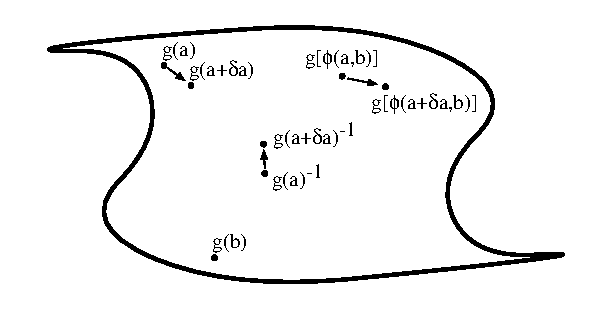
\includegraphics[scale=1.0]{pics/liejeva_mnogostrukost.eps}}
Tako teorija Liejevih grupa spaja ideje iz algebre, analize i geometrije.

Analiza općenitih Liejevih grupa, koja se oslanja samo na ovu definiciju
je matematički dosta zahtjevna. Srećom praktički sve Liejeve grupe koje se javljaju
u fizici mogu se vjerno reprezentirati matricama i mi ćemo se baviti
samo takvim tzv. matričnim Liejevim grupama. Smanjenje općenitosti je neznatno\footnote{Za
    znatiželjne, primjeri ne-matričnih Liejevih grupa su uvijek egzotični
    poput tzv. metaplektičkih grupa ili kvocijentne grupe Heisenbergove grupe po
jednoj svojoj specifičnoj normalnoj podgrupi.\label{fus:nematricne}},
a rad s matricama je značajno lakši od rada s diferencijabilnim mnogostrukostima.
Na primjer, matrice odmah dolaze parametrizirane brojčanim vrijednostima svojih
elemenata. Tu je važno
ne pomiješati dimezionalnost matrične grupe s dimenzionalnošću njenih matrica.
Kako je rečeno gore, dimenzionalnost grupe je jednaka broju \emph{nezavisnih realnih}
parametara koji specificiraju element grupe tj. matricu. Tako je grupa rotacija
u ravnini dana dvodimenzionalnim matricama
\begin{equation}
    \left\{ \begin{pmatrix}
        \cos\phi & -\sin\phi \\
        \sin\phi & \cos\phi 
    \end{pmatrix} 
     \td \phi \in [0, 2\pi) \right\} \,,
    \label{eq:so2}
\end{equation}
ali to je jednodimenzionalna grupa jer je svaka matrica potpuno određena
jednim realnim parametrom $\phi$. Matrične grupe imaju svoja klasična
imena pa se tako grupa iz (\ref{eq:so2}) zove \SO{2}, što dolazi
od \emph{specijalna} ($\det M = 1$) \emph{ortogonalna} ($M^\mathsf{T} M = 1$) 
grupa $2\times 2$ matrica.


\section{Grupe \SO{3} i \SU{2}}
\label{sec:so3su2}

Dva važna primjera Liejevih grupa na kojima  ćemo ilustrirati većinu rezultata
su grupa $3 \times 3$ ortogonalnih matrica determinante 1, dakle \SO{3},
i grupa $2 \times 2$ unitarnih matrica determinante 1, \SU{2}, pa ćemo
se u ovom odjeljku detaljnije upoznati s ove dvije grupe i njihovom
međusobnom vezom. No krenimo prvo
s malo općenitijim razmatranjem transformacija prostora koje
čuvaju udaljenosti između točaka.
Takve transformacije nazivaju se \emph{izometrije}. U vektorskim prostorima,
udaljenost točaka se prirodno definira kao norma razlike vektora do tih točaka,
pa će transformacije koje čuvaju skalarni produkt vektora $(\vec{x}, \vec{y})$,
čuvati i udaljenosti jer je norma (iznos) vektora $\sqrt{(\vec{x}, \vec{x})}$.
Zapišemo li to pomoću matrica vidimo da matrica izometrije $R$ mora zadovoljavati
\begin{equation}
    (R\vec{x}, R\vec{y}) = \sum_{ijk} R_{ij}x_{j} \, R_{ik} y_{k} = \sum_{ijk} x_{j} (R^\mathsf{T})_{ji}
    \, R_{ik} y_{k} = (\vec{x}, R^{\mathsf{T}} R \vec{y}) \stackrel{!}{=} (\vec{x}, \vec{y}) \,,
\end{equation}
pa mora biti $R^{\mathsf{T}} R = 1$, a matrice koje to zadovoljavaju
nazivamo \emph{ortogonalne} jer iz tog svojstva slijedi da su retci i stupci
tih matrica ortogonalni vektori, štoviše ortonormirani su. Grupa svih
ortogonalnih $3 \times 3$ matrica se naziva \O{3}.

Kako je prema Binet-Cauchyjevom teoremu $\det R^\mathsf{T} R = \det R^\mathsf{T} \det R$,
te kako transpozicija ne mijenja determinantu, vidimo da je $(\det R)^2 = 1$,
pa determinanta ortogonalne matrice može biti samo 1 ili -1. \label{pag:detO3}
Matrice s determinantom -1, poput 
\begin{equation}
\begin{pmatrix}
\cos\phi & -\sin\phi & 0 \\
\sin\phi & \cos\phi & 0 \\
0 & 0 & -1 \end{pmatrix} \,,
\end{equation}
daju transformacije koja su kombinacija rotacije i refleksije preko
neke ravnine kroz ishodište (u ovom primjeru to je $x$-$y$ ravnina).
Refleksije također čuvaju
udaljenosti, ali ne čuvaju orijentaciju (lijevi vijak se
se pretvara u desni). Podskup od \O{3} kojeg čine
matrice determinante 1 čini normalnu podgrupu (uvjerite se u to!)
koja se naziva \emph{specijalna} ortogonalna grupa \SO{3}.

Elementi komplementa od \SO{3} u \O{3} tj. matrice koje imaju determinantu -1 nekad se 
nazivaju \emph{neprave} rotacije.
Neprave rotacije se mogu na jedinstven
način prikazati kao umnožak običnih rotacija iz \SO{3} i operatora 
prostorne inverzije\footnote{Poznat i kao operator \emph{pariteta} zbog
    važnog svojstva parnosti kvantnomehaničkih valnih funkcija na transformaciju
prostorne inverzije.}
\begin{equation}
P = \begin{pmatrix}
-1 & 0 & 0 \\ 
0  &-1 & 0 \\
0  & 0 & -1
\end{pmatrix} \,.
\end{equation}
Naime, uzmemo li proizvoljnu nepravu rotaciju $\tilde{R}$ tada
je 
\begin{equation}
\det (P \tilde{R}) = \det(P) \det(\tilde{R}) = +1     
\end{equation}
pa je $P\tilde{R}$ 
prava rotacija, $P\tilde{R} = R$,
i onda je $\tilde{R} = P R$. Tako je cijeli taj skup
kojeg čine neprave rotacije zapravo jednak umnošku $P\SO{3}$ i vidimo da
se cijela ortogonalna grupa sastoji od točno dvije komponente
\begin{equation}
    \O{3} = \SO{3} + P\SO{3}\,,
    \label{eq:so3Pso3}
\end{equation}
od kojih je samo $\SO{3}$ podgrupa. ($P\SO{3}$ ne može biti podgrupa jer ne sadrži
jedinični element.)

Usredotočimo se sada na grupu $\SO{3}$ i promotrimo izgled njene grupne mnogostrukosti.
Svaki element grupe \SO{3} se može na jedinstven način definirati
smjerom osi rotacije i iznosom kuta rotacije pa se grupna mnogostrukost
može prikazati kao puna lopta promjera $\pi$ s identificiranim nasuprotnim
(antipodnim) točkama njene površine:

\centerline{\documentclass[border=3mm]{standalone}

\usepackage{tikz}
\usetikzlibrary{arrows.meta}
\usepackage{tikz-3dplot}

\begin{document}
	\tdplotsetmaincoords{15}{0}
	\begin{tikzpicture}[scale=1.5,tdplot_main_coords]
		\tdplotsetrotatedcoords{-45}{0}{0}
		\draw[very thick] (0,0) circle [radius=2cm];
		\draw[canvas is xz plane at y=0] (0,0) circle [radius=2cm];
		\draw[canvas is xz plane at y=0] (0,0) -- (2.5,0);
		\draw[canvas is xy plane at z=0] (0,0) -- (0,2.5);
		\draw[canvas is xy plane at z=0,tdplot_rotated_coords] (0,0) -- (0,1.5);
		
		\node[circle,inner sep=0pt,outer sep=2pt,fill=black,minimum size=3pt,label={left:$e$}] (1) at (0,0) {};
		\node[circle,inner sep=0pt,outer sep=2pt,fill=black,minimum size=3pt] (2) at (0,2cm) {};
		\node[circle,inner sep=0pt,outer sep=2pt,fill=black,minimum size=3pt] (3) at (0,-2cm) {};
		\node[circle,inner sep=0pt,outer sep=2pt,fill=black,minimum size=3pt] (4) at (1cm,0) {};
		\draw[Triangle-] (3) --++ (20:3cm) node[right,align=left] (5) {Rotacija oko\\
$z$-osi za $\pi$};
		\draw[Triangle-] (2) -- (5);
		\draw[Triangle-] (4) --++ (45:2cm) node[right,align=left] {Rotacija oko\\
$x$-osi za $\pi/2$};;
	\end{tikzpicture}
\end{document}}
%\centerline{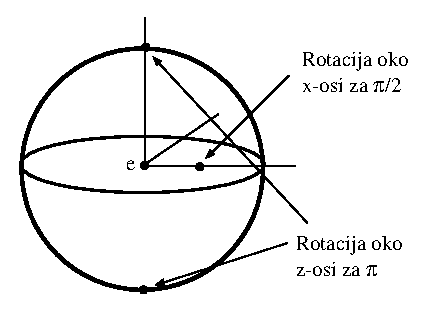
\includegraphics[scale=0.8]{pics/so3mnogostrukost.eps}}

Položaj točke u lopti dan je u sfernom koordinatnom sustavu kao
$(r, \theta, \phi)$. Kutovi $\theta$ i $\phi$ definiraju usmjerenje
osi rotacije, a udaljenost $r \le \pi$ točke od ishodišta definira kut rotacije.
Sve te rotacije uzimamo u pozitivnom smjeru. Rotacije u negativnom smjeru,
odnosno rotacije za 
kutove $(\pi, 2\pi)$ se dobiju rotacijom za kutove $[0, \pi]$ oko
suprotno usmjerene osi. Identifikacija nasuprotnih točaka je posljedica
činjenice da je su rotacije za $\pi$ oko suprotno usmjerenih osi
identične pa tek uz takvu identifikaciju imamo ispravnu bijekciju
između lopte (grupnog prostora) i \SO{3} grupe rotacija. 

Kompozicija u grupi \SO{3} je naravno dana umnoškom odgovarajućih matrica,
ali promatranjem rezultantne matrice općenito nije lako vidjeti kakvoj
rotaciji ona odgovara, za koji kut i oko koje osi. Odgovor na to pitanje,
kojim se nećemo ovdje baviti,
dali su Euler i Rodrigues, ali najelegantniji put do odgovora ide putem
grupe \SU{2} na koju ćemo se sada usredotočiti.
Da bismo ustanovili parametrizaciju grupe \SU{2}, a pomoću toga i izgled
njene grupne mnogostrukosti, promotrimo općenitu $2 \times 2$ kompleksnu
matricu
\begin{equation}
    U = 
    \begin{pmatrix}
        a & b \\ c & d
    \end{pmatrix} \,, \qquad
    a, b, c, d \in \mathbb{C} \,.
\end{equation}
Uvjet unitarnosti daje
\begin{equation}
    U U^\dagger = \begin{pmatrix}
        aa^*+bb^*  & ac^*+bd^* \\
        ca^*+db^* & c c^* + d d^*
    \end{pmatrix}
    \stackrel{!}{=}
    \begin{pmatrix}
        1 & 0 \\ 0 & 1
    \end{pmatrix} \,,
\end{equation}
dok uvjet specijalnosti daje
\begin{equation}
    \det U = ad - bc = 1 \,.
\end{equation}
Elimirajući $d$ iz jednadžbi $ca^*+db^* =0$ i $ad - bc = 1$ dobijemo
\begin{equation}
    -\frac{c}{b^*}(aa^* + bb^*) = 1 \,,
\end{equation}
pa kako je iz uvjeta unitarnosti $aa^* + bb^* = 1$ dobijemo da je $c=-b^*$.
Onda odmah iz $ca^*+db^* =0$ slijedi i da je $d = a^*$ pa vidimo da je
\begin{equation}
    \SU{2} = \left\{
        \begin{pmatrix}
            a & b \\ -b^* & a^*
    \end{pmatrix} \; \text{uz}\;   |a|^2 + |b|^2 = 1\,;\quad  a,b \in\mathbb{C} \right\} \,.
    \label{eq:su2ab}
\end{equation}
Ova dva kompleksna broja možemo izraziti preko realnih kao $a = x + iy$ i
$b = r + is$ čime uvjet determinante postaje
\begin{equation}
    x^2 + y^2 +r^2 +s^2 = 1 \,,
    \label{eq:s3sfera}
\end{equation}
i na kraju preostaju tri slobodna realna parametra. Dakle, grupa \SU{2} je troparametarska
ili trodimenzionalna Liejeva grupa. Parametre $x, y, r$ i $s$ možemo interpretirati
kao koordinate točaka u četverodimenzionalnom euklidskom prostoru $\mathbb{R}^4$
i kako je (\ref{eq:s3sfera}) jednadžba sfere u tom prostoru vidimo da je
grupna mnogostrukost grupe \SU{2} 3-sfera\footnote{Kružnica je 1-sfera $S^1$,
    Zemljina površina je približno 2-sfera $S^2$ itd. Interesantan vrlo
    netrivijalan rezultat teorije grupa je da od svih $S^n$ samo $S^1$ i $S^3$ dopuštaju
grupnu strukturu tj. mogu biti mnogostrukosti Liejeve grupe.} $S^3$.


Diskutirajmo sada vezu između grupa \SO{3} i \SU{2}. Za zagrijavanje, možemo
promotriti sličnu vezu jednostavnijih Abelovih grupa \SO{2} i \U{1}. Grupa \SO{2} je dana
u (\ref{eq:so2}), a \U{1} je grupa unitarnih $1 \times 1$
matrica, a to su naravno kompleksni brojevi apsolutne vrijednosti 1, jer uvjet
unitarnosti je $u^\dagger u = u^* u = |u| = 1$. Tako tu grupu možemo
parametrizirati kao $u = e^{i\phi}$, $\phi\in [0, 2\pi)$ i jasno je da je
i grupna mnogostrukost od \U{1} kružnica, kao i za \SO{2}. Štoviše ove dvije
grupe su očito izomorfne. Taj izomorfizam omogućuje da se mnogi
trigonometrijski identiteti ravninske geometrije, poput formula za sinus i kosinus dvostrukog kuta,
mogu znatno lakše izvesti u grupi \U{1} jer je s eksponencijalnom
funkcijom lakše raditi nego s trigonometrijskima, a na kraju se lako "vratimo
u \SO{2}" pomoću Eulerove formule $e^{i\phi} = \cos\phi + i\sin\phi$.

Kod grupa \SO{3} i \SU{2} situacija je ipak nešto složenija. Već smo vidjeli
da su grupne mnogostrukosti vrlo različite, a kako je
pokazano u Dodatku \ref{sec:su2so3} one
nisu izomorfne, nego samo homomorfne.
Konkretno, homomorfno preslikavanje je 2-na-1 tako da je svakim dvama elementima 
$U$ i $-U$ iz \SU{2} pridružen isti element $R$ iz \SO{3}.
Pomoću (\ref{eq:su2ab}) i (\ref{eq:s3sfera}) vidimo da množenje matrice $U$
s -1 odgovara promjeni parametara $(x, y, r, s) \to (-x, -y, -r, -s)$,
što je inverzija u 4D prostoru, tako da elementima $U$ i $-U$ odgovaraju
antipodne točke na grupnoj mnogostrukosti $S^3$. No, za razliku od
grupne mnogostrukosti \SO{2} gdje su antipodne točke površine kugle
identificirane i odgovaraju jednom elementu grupe, ovdje su antipodne
točke različite i odgovaraju različitim elementima grupe.
Zahvaljujući ovom homomorfizmu, rotacije u 3D prostoru mogu se reprezentirati
i matricama iz SU(2), a ova prividna redundancija dvaju matrica za
istu rotaciju s pokazuje ključna u kvantnoj mehanici sustava s polucjelobrojnim
spinom, kako ćemo vidjeti u \ref{ch:rotacije}. poglavlju.

Kernel ovog homomorfizma je znači $\{\mathbb{I}, -\mathbb{I}\}$ što je
grupa $\mathbb{Z}_2$ pa prema
teoremu o izomorfizmu \ref{th:izomorfizam} imamo
odnos $\SU{2}/\mathbb{Z}_2 = \SO{3}$.





\section{Liejeve algebre}
\label{sec:liejevealgebre}

Promotrimo sada skup matrica $M(a)\equiv M(a_1, a_2, \ldots, a_n)$ koje
čine $n$-pa\-ra\-me\-tar\-sku Liejevu grupe.
Za infinitezimalno male vrijednosti parametara $a_i \to \epsilon_i \ll 1$, zahvaljujući
svojstvu diferencijabilnosti Liejeve grupe možemo razviti oko $a_i = 0$:
\begin{equation}
   M(\epsilon)=M(0)+ \sum_{i=i}^{n}\epsilon_i \frac{\partial M(a_1, \ldots, a_n)}
 {\partial a_i}\Bigg|_{a_1=\ldots =a_n=0} + 0(\epsilon^2) \,,
 \label{eq:razvojM}
\end{equation}
gdje diferenciranje matrica provodimo prirodno diferencirajući svaki njen
element ponaosob. Koeficijenti od $\epsilon_i$ u (\ref{eq:razvojM}) su
konstantne matrice (ne ovise o parametrima) koje se nazivaju generatori
i skraćeno ćemo ih označiti s $X_i$
\begin{equation}
X_i =  \frac{\partial M(a_1, \ldots, a_n)}
 {\partial a_i}\Bigg|_{a_1=\ldots =a_n=0} = \textrm{const}(a_1, \ldots, a_n)
   \quad i=1, \ldots, n 
   \label{eq:defXi}
\end{equation}
Očito je da generatora ima koliko i parametara tj. njihov broj je jednak
dimenzionalnosti grupe (grupne mnogostrukosti).  $M(0)$ je jedinični
element grupe tj. jedinična matrica pa za infinitezimalne transformacije imamo
\begin{equation}
  M(\epsilon)=\Eins + \sum_{i=i}^{n}\epsilon_i X_i \,. 
\end{equation}

Centralna spoznaja teorije Liejevih grupa je da je struktura \emph{čitave} grupe i
njenih reprezentacija skoro sasvim određena
određena generatorima grupe tj. infinitezimalnom okolinom jediničnog 
elementa.
Ovo ćemo većim dijelom samo pokazati na primjeru grupe rotacija realnog
trodimenzionalnog euklidskog prostora, a za općeniti
dokaz čitaoc može konzultirati literaturu poput \cite{Stilwell:2008}.


U odjeljku \ref{sec:primjeriLie} dokazat ćemo da je grupa \SO{3} troparametarska,
no to je i odmah jasno ako znamo da su rotacije potpuno specificirane pomoću
iznosa kuta rotacije (jedan parametar) i usmjerenja jediničnog vektora osi rotacije (dva parametra)
ili alternativno pomoću tri Eulerova kuta.

Promotrimo sada jednoparametarsku podgrupu grupe \SO{3} koju čine
rotacije oko treće tj. $z$-osi.
\begin{displaymath}
\left\{ R_3 (\phi) = 
\begin{pmatrix}
\cos\phi & -\sin\phi & 0 \\
\sin\phi & \cos\phi & 0 \\
0 & 0 & 1 
\end{pmatrix}
 \td \phi \in [0, 2\pi) \right\} = \SO{2} \subset \SO{3} \,,
\end{displaymath}
gdje premda su same matrice $R_3 (\phi)$ trodimenzionalne one su
naravno izomorfne grupi \SO{2} rotacija $x$-$y$ ravnine.
Generator te pogrupe je
\begin{equation} \label{eq:x3so3}
X_3 = \frac{\partial R_3 (\phi)}{\partial \phi}\Bigg|_{\phi=0}=
\begin{pmatrix}
-\sin\phi & -\cos\phi & 0 \\
\cos\phi & -\sin\phi & 0 \\
0 & 0 & 1 
\end{pmatrix}\Bigg|_{\phi=0} =
\begin{pmatrix}
0 & -1 & 0 \\
1 & 0 & 0 \\
0 & 0 & 0 
\end{pmatrix} \,,
\end{equation}
i infintezimalna rotacija oko $z$-osi je $R_3 (\epsilon) = 1 + \epsilon X_3$.
Ideja je sada komponirati $N$ ovih rotacija za infinitezimalni kut
$\epsilon$ i uočiti da
će u limesu $N \to\infty$ uz $N\epsilon \to \phi$ 
takva kompozicija rezultirati rotacijom za proizvoljni \emph{konačni}
kut $\phi$
\begin{displaymath}
[R_3(\epsilon)]^{N} = (1+\epsilon X_3)^N = \left(1+\frac{(N\epsilon)X_3}
 {N}\right)^N 
 \xrightarrow[\substack{N \to \infty \\ (N\epsilon) \to \phi}]{}
 e^{\phi X_3} \,,
\end{displaymath}
gdje smo upotrijebili svojstvo eksponencijalne funkcije
\begin{equation}
    \lim_{N\to\infty}\left(1 + \frac{x}{N}\right)^N = \exp(x) \,,
\end{equation}
koje vrijedi za broj $x$,
u nadi da će ono vrijediti i kad je $x$ matrica.
U dodatku \ref{sec:expmat} diskutiramo
kako eksponenciranje matrica zaista funkcionira isto kao i
eksponenciranje brojeva, uz još neka dodatna zanimljiva svojstva,
te tamo usput eksplicitno pokazujemo da je
\begin{equation}
e^{\phi X_3} = \exp\Bigg\{ 
    \phi  \begin{pmatrix}
0 & -1 & 0 \\
1 & 0 & 0 \\
0 & 0 & 0 
\end{pmatrix}\Bigg\} =
\begin{pmatrix}
\cos\phi & -\sin\phi & 0 \\
\sin\phi & \cos\phi & 0 \\
0 & 0 & 1 \end{pmatrix} \,.
\end{equation}
Tako vidimo da zaista svaki element ove jednoparametarske podgrupe
od \SO{3} možemo dobiti eksponencijacijom generatora.
Nadalje, u skladu s Eulerovim teoremom iz mehanike\footnote{Svaki pomak krutog
tijela kod kojeg jedna točka ostaje nepomična je ekvivalentan \emph{jednoj}
rotaciji oko fiksne osi koja prolazi kroz tu točku.} svaka \SO{3} rotacija 
pripada nekoj jednoparametarskoj podgrupi
 (čine je sve rotacije oko te iste osi), što onda znači da se
svi elementi grupe \SO{3} mogu se dobiti eksponencijacijom generatora.
Mogućih osi rotacije ima beskonačno pa tako i geratora ima beskonačno
i pitanje je kako ih odrediti.
Kako se vidi iz (\ref{eq:defXi}) konkretan oblik generatora ovisi
o parametrizaciji grupnog prostora. 
Mogli bismo recimo pokušati konstruirati opću rotaciju kao kompoziciju tri
 Eulerove rotacije i onda deriviranjem po Eulerovim kutovima dobiti
 generatore. No, ima i lakši put koji će olakšati traženje 
 generatora drugih Liejevih grupa koje se pojavljuju u fizici\footnote{Recimo
     usput i da bi pristup preko Eulerovih
     bio  problematičan jer su one singularne oko jedinice.}.

Oslonit ćemo se na definiciju \SO{3} kao grupe svih 
3$\times$3 matrica $R$ sa svojstvom  $RR^\mathsf{T}=1$ i $\det R=1$.
Rotacije za infinitezimalni kut imat će oblik  $R(\epsilon)=1+\epsilon X$,
gdje je $X$ jedan od generatora. Uvjet ortogonalnosti je sada
\begin{equation} \label{eq:Xantisim}
 RR^\mathsf{T}=(1+\epsilon X)(1+\epsilon 
   X^\mathsf{T}) = 1+\epsilon (X+X^\mathsf{T})+0(\epsilon^2) = 1 \,,
\end{equation}
što znači da je $X^\mathsf{T}=-X$ odnosno $X$ je antisimetrična 3$\times$3 matrica.
Obratno, ako je $X$ antisimetrična, njena eksponencijacija $R = e^X$ daje ortogonalnu
matricu jer je
\begin{equation}
  R R^\mathsf{T} = e^X (e^X)^\mathsf{T} = e^X e^{X^\mathsf{T}}
  = e^X e^{-X}
  = e^{X-X} = 1 \,,
\end{equation}
gdje je jedini netrivijalni korak predzadnji. Naime, vidi dodatak \ref{sec:expmat},
$e^{A} e^{B} = e^{A+B}$ samo ukoliko matrice $A$ i $B$ komutiraju što je ovdje
srećom trivijalno slučaj.
Zahvaljujući općenitoj relaciji $\det e^{X} = e^{\textrm{\scriptsize Tr} X}$,
vidi dodatak \ref{sec:expmat}, te činjenici da antisimetrične matrice imaju
nule na glavnoj dijagonali, uvjet specijalnosti determinante $\det R = 1$ je
zadovoljen automatski.
Tako smo pokazali da skup $\calA$ svih antisimetričnih 3$\times$3 matrica
generira grupu \SO{3}\footnote{Pažljivi čitaoc će možda u ovom automatskom
    zadovoljenju uvjeta $\det R =1$ vidjeti kontradikciju:
 Refleksije su isto ortogonalne matrice,
pa bi i njihovi generatori trebali biti antisimetrični, no njihova determinanta
je -1. Stvar je u tome da refleksije nije moguće generirati kompozicijom
infinitezimalnih transformacija tj. one nemaju generatore. O tome će još biti
govora kasnije.\label{fus:refleksija}
}.

Skup generatora $\calA$ ima i dodatna svojstva. Kao prvo, on je
vektorski prostor nad poljem $\mathbb{R}$ jer za svaka dva vektora
$X_1, X_2\in\calA$ i svaka dva broja $\alpha, \beta\in\mathbb{R}$ 
$(\alpha X_1 + \beta X_2)$ je isto antisimetrična matrica, a time i
element $\calA$. Dimenzija od $\calA$ je 3 jer je najopćenititiji
oblik $3\times 3$ antisimetrične matrice
\begin{equation}
    \begin{pmatrix}
        0 &  a  &  b \\
       -a &  0  &  c \\
       -b & -c  &  0
   \end{pmatrix}  \qquad   a, b, c \in \mathbb{R} \,.
\end{equation}
Jednakost dimenzija vektorskog prostora generatora $\calA$ i grupe \SO{3} koju
oni generiraju naravno nije slučajna obzirom da eksponencijacijom
generatora trebamo moći dobiti skoro sve elemente grupe, a u najmanju ruku
barem sve elemente u nekoj okolini jedinice.

Trodimenzionalni vektorski prostor ima tročlanu bazu i u ovom slučaju je
uobičajeno kao bazu izabrati generatore jednoparametarskih podgrupa rotacija oko
$x$, $y$ i $z$ osi. Ovaj treći smo već odredili u (\ref{eq:x3so3}), a kompletna
baza je
\begin{equation}
X_1=
\begin{pmatrix}
0 & 0 & 0 \\ 
0 & 0 &-1 \\
0 & 1 & 0
\end{pmatrix}  \quad
X_2=
\begin{pmatrix}
0 & 0 & 1 \\ 
0 & 0 & 0 \\
-1& 0 & 0
\end{pmatrix}  \quad
X_3=
\begin{pmatrix}
0 & -1 & 0 \\ 
1& 0 & 0 \\
0 & 0 & 0
\end{pmatrix} \,,
\label{eq:SO3generators}
\end{equation}
pa je $e^{\phi \vec{X}\cdot\unitn}$ onda općeniti element grupe \SO{3} koji
predstavlja rotaciju oko osi $\unitn$ za kut $\phi$.

Vektorski prostor sa svojom dodatnom operacijom množenja
skalarima iz polja $\mathbb{R}$ je općenito znatno bogatija struktura od grupe (koja
ima samo svoju binarnu operaciju). To znači da o generatorima "znamo više" i
lakše je proučavati njih i onda pomoću eksponencijacije vidjeti reperkusije tih
spoznaja na samu grupu.
To je dodatno pojačano još jednim njihovim važnim svojstvom.
Neka su $X,Y\in\calA$. Definirajmo njihov \emph{komutator} 
\begin{equation}
    [X, Y] \equiv X Y - Y X \,.
    \label{eq:defkomutator}
\end{equation}
Komutator je također $3\times 3$ matrica koja je štoviše također antisimetrična
jer
\begin{equation}
 [X,Y]^\mathsf{T} = (XY-YX)^\mathsf{T} = Y^\mathsf{T} X^\mathsf{T} - X^\mathsf{T} Y^\mathsf{T}
 = YX-XY = -[X,Y] \,.
\end{equation}
To znači da je i komutator $[X,Y]\in\calA$.
Dakle, $\calA$ je zatvoren ne samo obzirom na linearne kombinacije već
i obzirom na komutatore svojih elemenata. Time je on još složenija matematička
struktura od vektorskog prostora koja se naziva  \emph{Liejeva algebra}.
Načinimo kratki odmak od proučavanja samo matričnih grupa i
definirajmo Liejevu algebru nešto općenitije.
\begin{definicija}[Liejeva algebra]
Liejeva algebra $\calA$ je vektorski prostor na kojem je definiran 
Liejev produkt dvaju elemenata $[X,Y]$ (ne mora biti komutator) sa svojstvima

1) zatvorenost: $[X,Y]\in\calA \quad \forall X,Y\in\calA$

2) distributivnost: $[\alpha X + \beta Y, Z]=\alpha[X,Z]+\beta[Y,Z]$
$\quad \alpha,\beta \in \mathbb{R} $

3) antisimetrija: $[X,Y]=-[Y,X]$

4) Jacobijev identitet: $[X, [Y, Z]]+[Y, [Z, X]]+[Z, [X, Y]]=0$
\end{definicija}
Za vektorske prostore matrica, gdje je Liejev produkt definiran kao
komutator (\ref{eq:defkomutator}), svojstva 2--4 su automatski ispunjena.
Ovo poopćenje od matričnih grupa smo napravili samo zato da kao
spomenemo da zapravo o nikakvom poopćenju nema govora.
Naime, kako smo rekli u fusnoti na stranici \pageref{fus:nematricne}, nematrične Liejeve grupe
su egzotične, ali postoje. No, zahvaljujući sljedećem Adovom teoremu
nematrične (konačno-dimenzionalne) Liejeve algebre ne postoje.
\begin{teorem}[Ado]
 Svaka konačno-dimenzionalna apstraktna Liejeva algebra je izomorfna nekoj
 Liejevoj algebri konačno-dimenzionalnih matrica s komutatorom kao Liejevim produktom. \emph{(Bez
 dokaza.)}
\end{teorem}
Dakle, ograničavajući se na Liejeve grupe \emph{matrica} ne gubimo mnogo
na općenitosti jer sve Liejeve algebre koje ćemo sresti u ovoj knjizi su
konačno-dimenzionalne\footnote{Istina, u fizici nekad nalazimo i primjenu beskonačno-dimenzionalnih
algebri za koje teorem ne vrijedi. Jedan primjer je tzv. Virasorova algebra važna
u teoriji superstruna.}.
Liejeve algebre se obično označavaju isto kao i pripadajuće Liejeve grupe, ali malim gotičkim slovima.
Dakle, $\calA = \soAlg{3}$.

Komutatori elemenata baze Liejeve algebre $X_i, i=1,2,\ldots, \textrm{dim}(\calA)$ se
kao i svi ostali elementi od $\calA$ naravno mogu prikazati kao linearna kombinacija baze, dakle
sebe samih: 
\begin{equation}
 [X_i, X_j]= \sum_k C_{ij}^{k} X_k \,,  \qquad i,j=1,2,\ldots, \textrm{dim}(\calA) \,.
 \label{eq:defstrukturne}
\end{equation}
Realni brojevi $C_{ij}^{k}$ koji se ovdje pojavljuju nazivaju se \emph{strukturne konstante} grupe.
Uočite da je (\ref{eq:defstrukturne}) vrlo netrivijalna nelinearna relacija između
generatora koju će morati zadovoljavati sve njihove reprezentacije.  Naime, cijelo ovo
izlaganje dosad koristilo je $3\times 3$ matrice za definiciju grupe \SO{3} i njene
algebre \soAlg{3}. To je istovremeno i definicija te grupe i reprezentacija te grupe 
na 3D euklidskom prostoru.
Međutim, slično kao i kod konačnih grupa, Liejeve grupe imaju i
reprezentacije na vektorskim prostorima drugih dimenzionalnosti, što je od velike
važnosti u primjeni teorije grupa na kvantnomehaničke sustave. I tu će opet biti od interesa
identificirati sve ireducibilne reprezentacije neke grupe. Koliko ireducibilnih
reprezentacija očekujemo? Ako bismo se oslonili na fundamentalni rezultat iz teorije
konačnih grupa da ireducibilnih reprezentacija ima isto koliko i klasa konjugacije,
vidi odjeljak \ref{sec:ortogonalnost}, onda bismo zaključili da \SO{3} ima beskonačno
ireducibilnih reprezentacija (jer se uz malo geometrijskog razmišljanja lako uvjerite
da pojedinu klasu konjugacije čine rotacije oko bilo koje osi za konkretni kut $\phi$).
I premda je takvo zaključivanje nekorektno jer navedena jednakost broja ireducibilnih
reprezentacija i klasa konjugacije \emph{ne vrijedi} za Liejeve grupe, zaključak jest
točan --- Liejeve grupe tipično imaju beskonačno ireducibilnih reprezentacija.
Jedna od lako uočljivih razlika prema konačnim grupama je u tome da premda
\SO{3} ima neprebrojivo beskonačno klasa konjugacije, vidjet ćemo da ima samo prebrojivo
beskonačno ireducibilnih reprezentacija.
Bez obzira, očito je da nećemo moći eksplicitno konstruirati sve te repreprezentacije
metodom nadopunjavanja tablice karaktera iz odjeljka \ref{sec:karakteri},
nego apstraktnijim zaključivanjem u kojem će
relacija (\ref{eq:defstrukturne}), koju fizičari često zovu "algebra grupe," imati
centralnu ulogu, kako ćemo vidjeti u sljedećim poglavljima.
Kad smo već kod terminologije, recimo i to da je fizičarima često interes usredotočen
samo na bazu Liejeve algebre, a ne i na ostatak vektorskog prostora, pa će u žargonu
reći da tri matrice iz (\ref{eq:SO3generators}) "čine algebru" ove grupe.


\begin{primjer}[strukturne konstante od \SO{3}]
Eksplicitnim računom lako se uvjerimo da je
 \begin{align}
     [X_i,X_j]& =0 \quad\text{za}\quad i=j \,,  \\
     [X_1,X_2]& = X_3 \,, \\
     [X_2,X_3]& = X_1  \,, \\
     [X_3,X_1]& = X_2 \,,
 \end{align}
tj. da je
\begin{align}
 C_{ij}^{k}& = 0 \quad\text{ako su bilo koja dva indeksa ista} \,, \\
 C_{12}^3  & = C_{23}^{1}=C_{31}^{2}=1 \,, \\
 C_{21}^3  & = C_{32}^{1}=C_{13}^{2}=-1 \,, \\
 \end{align}
pa pomoću Levi-Civita tenzora
komutacijske relacije algebre \soAlg{3} možemo zapisati u obliku
\begin{equation}
 [X_i, X_j]=\epsilon_{ijk} X_k  \,,
  \label{eq:algebraso3}
\end{equation}
odnosno strukturne konstante grupe \SO{3} su $C_{ij}^{k} = \epsilon_{ijk}$.
\end{primjer}


Liejeva algebra $\calA'$ je \emph{homomorfna} Liejevoj algebri $\calA$ ako postoji 
matrica $S:\calA\to\calA'$ takva da je
\begin{displaymath}
       [S(X), S(Y)]=S([X,Y]) \quad \forall X, Y \in\calA \,.
\end{displaymath}
Ako je $S$ još i bijekcija $\calA$ i $\calA'$ su \emph{izomorfne}. Dakle,
važno je da preslikavanje  bude konzistentno s operacijom komutatora.

\begin{primjer}[Liejeva algebra grupe \SU{2} tj. \suAlg{2}] \label{pr:su2so3Alg}
    \SU{2} je grupa svih unitarnih $2\times 2$ matrica jedinične determinante.
    Identičnim zaključivanjem kao za \SO{3}, samo uz zamjenu traspozicije
    hermitskom konjugacijom $X^\mathsf{T} \to X^\mathsf{\dagger}$ lako
    zaključujemo da algebru \suAlg{2} čine sve
    antihermitske\footnote{$A$ je antihermitska ako je $A^\dagger=-A$} 
    2$\times$2 matrice s tragom nula (ovdje zadovoljavanje uvjeta jedinične
    determinante nije automatsko). Kao bazu ove algebre uzimamo
\begin{equation}
     \{ -i\frac{\sigma_1}{2},  -i\frac{\sigma_2}{2},  -i\frac{\sigma_3}{2} \} \,,
\end{equation}
gdje su $\sigma_{1,2,3}$ tri Paulijeve matrice
\begin{equation}
\sigma_1=\left( \begin{array}{cc} 0 &  1 \\ 1 & 0 \end{array} \right) \,,
\quad
\sigma_2=\left( \begin{array}{cc} 0 & -i \\ i & 0 \end{array} \right) \,,
\quad
\sigma_3=\left( \begin{array}{cc} 1 &  0 \\ 0 &-1 \end{array} \right) \,.
\label{eq:PaulijeveMatrice}
\end{equation}
Ova tri generatora zadovoljavaju identične komutacijske relacije kao i matrice
\soAlg{3} algebre
\begin{displaymath}
 \left[ -i\frac{\sigma_1}{2}, -i\frac{\sigma_2}{2} \right] =
 -i\frac{\sigma_3}{2} \qquad \text{itd.}
\end{displaymath}
pa je pridruživanje $X_i \to -i \sigma_i/2$  izomorfizam i
\soAlg{3}=\suAlg{2}.

Važno je ovdje uočiti da premda su elementi matrica iz \suAlg{2} općenito kompleksni,
\suAlg{2} je \emph{realna} Liejeva algebra, dakle algebra nad poljem $\mathbb{R}$. 
(Linearna kombinacija $\sigma_1 + \sigma_2$ je antihermitska i time pripada \suAlg{2},
dok $\sigma_1 + i \sigma_2$ to nije!)

Zanimljivo je pitanje što izomorfizam algebri znači za odgovarajuće grupe tj.
jesu li možda onda i \SO{3} i \SU{2} izomorfne. O tome će biti riječi u sljedećem odjeljku.
\end{primjer}

Pri analizi reprezentacija Liejevih grupa od koristi će biti
tzv. Casimirovi operatori.
\begin{definicija}[Casimirov operator]
Ako je skup $\{X_i, i=1,2, ... \}$ baza Liejeve algebre onda se polinom
u $X_i$ koji komutira sa svim elementima te algebre naziva 
\emph{Casimirov operator}.
\end{definicija}
Posebno su zanimljivi kvadratični Casimirovi operatori.
\begin{primjer}[Kvadratični Casimirov operator za \soAlg{3} i \suAlg{2}]
 Eksplicitnim računom se uvjerimo da je 
\begin{equation}
X_{1}^2 + X_{2}^2 + X_{3}^2 = -2\cdot \Eins \,,
\end{equation}
    za \soAlg{3} i
\begin{equation}
    \left(\frac{-i}{2}\right)^2
    \big(\sigma_{1}^2 + \sigma_{2}^2 + \sigma_{3}^2\big) = -\frac{3}{4} \cdot \Eins \,,
\end{equation}
    za \suAlg{2}.
\end{primjer}
Schurova lema, koja vrijedi i za Liejeve grupe, traži da Casimirov operator 
bude proporcionalan jediničnom i ispostavlja se da je koeficijent proporcionalnosti
zgodan za označavanje ireducibilnih reprezentacija kako ćemo vidjeti u sljedećem poglavlju.


\begin{primjer}[Algebra grupe \SO{2}]
    Generator grupe \SO{2} već smo identificirali kao $X_3$ iz
    \ref{eq:x3so3} kad smo \SO{2}
    razmatrali kao jednoparametarsku podgrupu grupe \SO{3}.
    No kakva je struktura njene algebre? Ona je generirana tim
    jednim generatorom koji naravno komutira sa samim sobom
    tj. $\soAlg{2} = \{ aX_{3}\,; a \in \mathbb{R} \}$, što je
    zapravo prostor svih antisimetričnih $2\times 2$ matrica,
    koji je izomorfan s $\mathbb{R}$.
    Općenito, za Liejeve algebre Abelovih grupa komutator iščezava 
    (vidi zadatak \ref{zad:abelovaalgebra}) i time
    je njihova struktura kompletno definirana strukturom vektorskog
    prostora. \label{pr:so2Alg}
\end{primjer}


\section{Veza Liejevih grupa i Liejevih algebri}

Vidjeli smo da u slučaju grupe \SO{3} 
\emph{svaki} element grupe možemo prikazati kao eksponencijal nekog
elementa njene Liejeve algebre \soAlg{3}.
Pitanje je vrijedi li to lijepo svojstvo za sve Liejeve grupe.
Kako smo već dali naslutiti na nekoliko mjesta upotrijebom riječi "skoro",
ne vrijedi sasvim. U ovom ćemo odjeljku, uglavnom
bez dokaza, iskazati i pomoću primjera ilustrirati tvrdnje koje 
pobliže oslikavaju vezu između Liejevih grupa i njihovih algebri.
Za većinu primjena u fizici i u ostatku knjige, uglavnom ćemo
se fokusirati na algebre i reprezentacije algebri, tako da (razmjerno
zahtjevno) gradivo ovog odjeljka nije nužno za razumijevanje sljedećih
poglavlja.

Prvo je potrebno uvesti neke pojmove koji opisuju topološka
svojstva grupe.
\begin{definicija}[Povezanost]
Liejeva grupa je \emph{povezana} ako njen grupni prostor ne možemo
rastaviti na disjunktne komponente tj. ako se svake dvije točke 
mogu povezati linijom čije sve točke pripadaju grupnom prostoru.
(Ovo je intuitivna "fizičarska" definicija. Prava definicija uključuje napredne
matematičke ideje iz topologije.)
\label{def:povezanost}
\end{definicija}
Podskup kojeg čine svi elementi grupe koji se
kontinuiranom linijom u grupnoj mnogostrukosti mogu povezati s
jediničnim elementom nazivamo \emph{komponenta povezanosti jedinice}.
Ukoliko je grupa povezana komponenta povezanosti jedinice je naravno
jednaka cijeloj grupi. Ukoliko grupa nije povezana, komponenta povezanosti
jedinice je prava podgrupa cijele grupe. \emph{Dokaz}: Pretpostavimo
suprotno tj. da komponenta povezanosti jedinice nije podgrupa. Kako je
jedinični element po definiciji u toj komponenti te kako je asocijativnost
nasljeđena od cijele grupe to bi značilo ili da postoje njena dva elementa čiji
umnožak nije u komponenti povezanosti jedinice ili neki element čiji inverz nije u 
toj komponenti.
Promotrimo sada dva elementa $a$ i $b$ koji jesu, a čiji umnožak $ab$ nije u komponenti
povezanosti jedinice, te promotrimo trajektoriju $g(t)$, $t\in[0,1]$,
definiranu tako da je $g(0)=a$, a $g(1)=e$. Trajektorija dakle
kontinuirano povezuje $a$ s jediničnim elementom $e$.
Pomičući se kontinuirano po toj trajektoriji prema jedinici
umnožak $g(t)b$ će cijelo vrijeme ostati izvan komponente povezanosti jedinice
zbog odvojenosti njegovog dijela grupnog prostora i kontinuiranosti
funkcije kompozicije (umnožak $g(t)b$ ne može "preskočiti" sa svoje odvojene
komponente na komponentu jedinice). No kad dođemo do jediničnog elementa
umnožak je $g(1)b = eb = b$ što po pretpostavci jest element komponente jedinice
i imamo kontradikciju. Na sličan način se do kontradikcije dođe u slučaju inverza.\qed

Eksponencijacijom generatora grupe \SO{3} dolazimo do konačnih rotacija
$\exp(\phi \vec{X}\cdot\unitn)$ trajektorijom koja ide od jediničnog
elementa $\phi=0$ kontinuiranom putanjom kroz grupni prostor, kompozicijom rotacija za
infinitezimalne kuteve. Kako je eksponencijalna funkcija kontinuirana
funkcija svojih argumenata (čak i kad su argumenti matrice), te kako
je determinanta također kontinuirana funkcija, u slučaju grupe \O{3},
za čije elemente smo vidjeli da imaju determinantu ili +1 ili -1,
jasno je da eksponencijacijom algebre možemo dobiti (a u slučaju \O{3}
i dobivamo) samo elemente s determinantom +1, dakle prave rotacije.
Neprave rotacije $I\SO{3}$ koje imaju determinantu -1
pripadaju drugoj komponenti povezanosti. \label{pag:povezanostO3}



Iz gornje diskusije, odnosno imajući u vidu kontinuiranost funkcije
eksponencijacije, jasno da najbolje čemu se možemo nadati u
slučaju općenite Liejeve grupe je da
eksponencijacijom njene algebre dobijemo komponentu povezanosti
jedinice. No je li barem to uvijek moguće?
Kako smo pokazali, svakoj Liejevoj grupi jednoznačno pripada neka Liejeva algebra
konstrukcijom kao u (\ref{eq:defXi}). Možemo li, obratno, svakom
elementu $g$  komponente povezanosti jedinice pridružiti jedinstveni
element $X$ algebre takav da je $g = e^{X}$?

Prije nego damo odgovor na to pitanje, skrenimo pažnju na to da je
povezivanje elemenata algebre i elemenata grupe exponencijacijom
(odnosno u drugom smjeru inverznom funkcijom logaritma) samo dio
posla. Potrebno je pokazati i da je binarna grupna operacija potpuno
određena operacijama s odgovarajućim elementima algebre. Kako
dakle izračunati $e^X e^Y$? Imajuči u vidu definiciju eksponencijacije
to je
\begin{equation}
   e^X e^Y = \left(\sum_{k=0}^{\infty} \frac{X^k}{k!}\right)
             \left(\sum_{n=0}^{\infty} \frac{Y^n}{n!}\right)
    \,,
\end{equation}
i nije odmah jasno da se desna strana može dobiti eksponencijacijom nekog
elementa algebre, osim u jednostavnom slučaju Abelove grupe kad je 
$[X, Y]=0$ (vidi zadatak \ref{zad:abelovaalgebra}) pa se članovi
gornjih suma mogu isto kao kod eksponencijacije običnih brojeva
iskombinirati u $\sum (X+Y)^{n}/n! = \exp(X+Y)$. Za općenite
nekomutirajuće grupe to nije slučaj, nego vrijedi sljedeći važan
rezultat teorije Liejevih grupa
\begin{teorem}[Baker-Campbell-Hausdorff] \label{th:bch}
    \[ e^X e^Y = e^Z \,, \]
  gdje je 
  \[ Z = X + Y + \text{red višestrukih komutatora $X$ i $Y$.} \]
\end{teorem}
Prvi članovi BCH formule su
\begin{align}
    Z& = X + Y + \frac{1}{2}[X, Y] + \frac{1}{12}[X, [X, Y]] 
       - \frac{1}{12}[Y, [X, Y]] \nonumber \\
     &   - \frac{1}{24}[X, [Y, [X, Y]]] + \frac{1}{720}[Y, [Y, [Y, [X, Y]]]] 
         + \cdots \,,
   \label{eq:bch}
\end{align}
i ključna netrivijalnost je da su \emph{svi} članovi reda dati preko
ovakvih višestrukih komutatora pa je jasno da je $Z$ element Liejeve algebre.
(Podsjetimo se da je u Liejevoj algebri definirano zbrajanje elemenata $X+Y$ i njihov
 komutator $[X, Y]$, ali ne i množenje\footnote{Ako gledamo matrične
    Liejeve algebre množenje samih matrica jest definirano, ali algebra općenito nije zatvorena
    na to množenje. Npr. umnožak dvije antisimetrične matrice iz \soAlg{3} 
    općenito \emph{nije} antisimetrična matrica.} $X Y$.)
BCH red konvergira u nekoj okolini jediničnog elementa (ne nužno infinitezimalnoj)
i u toj okolini je grupa potpuno i jedinstveno određena algebrom.
Eksponencijacija povezuje elemente grupe i algebre, a BCH formula
operacije u algebri (zbrajanje i komutator) s grupnom operacijom (množenje).
Dokaz teorema \ref{th:bch}  i razmatranje radijusa konvergencije BCH formule (\ref{eq:bch}) 
obično zahtijeva napredne matematičke
pojmove. Relativno pristupačan algebarski dokaz može se pronaći
u \cite{Stilwell:2008}.

Za veliku kategoriju Liejevih grupa vrijedi da se svi elementi iz 
komponente povezanosti jedinice mogu prikazati u obliku
$e^{X}$ gdje je $X$ element
Liejeve algebre. Dovoljan uvjet je da grupa ima svojstvo \emph{kompaktnosti}.
\begin{definicija}[Kompaktnost]
Liejeva grupa je \emph{kompaktna} ako njeni parametri variraju po zatvorenim intervalima.
(Ovo je intuitivna "fizičarska" definicija. Prava definicija uključuje napredne
matematičke ideje iz topologije.)
\label{def:kompaktnost}
\end{definicija}
Mnoge grupe koje će nas interesirati, poput
\SO{n} i \SU{n} su kompaktne, jer njihovi parametri tipično variraju
po intervalima poput $\phi \in [0, 2\pi)$. Iznimka je
grupa translacija, čiji parametri variraju po intervalu $(-\infty,
\infty)$ i grupa Lorentzovih transformacija, čiji parametar
potiska varira $v \in [0, c)$, gdje $c$ nije uključen i stoga
je interval otvoren i nekompaktan\footnote{Radi
    kompletnosti spomenimo da ako Liejeva grupa nije kompaktna, 
    svejedno se elementi iz komponente
povezanosti jedinice mogu prikazati kao konačan umnožak eksponencijala
$e^{X_1} e^{X_2}\cdots e^{X_n}$ \cite{Stilwell:2008}.
Treba razlikovati situaciju gdje se svaki element
grupe (ili njenog podskupa) može dobiti eksponencijacijom (exp
je surjektivna) i situaciju gdje se on može se dobiti na jedinstven način 
(exp je i injektivna).
Injektivnost je zahtjevnije svojstvo. 
Treba uočiti da se algebra grupe \SO{2} preslikava na grupu neinjektivno,
pa nijedna grupa koja
je sadrži kao podgrupu, kao \SO{3}, \SU{2} etc., neće biti injektivno pokrivena
exponencijacijom. Surjektivnost je lakše postići.
Za to je dovoljna kompaktnost,
a može i niže definirana jednostruka povezanost.}.


Dakle, Liejeva algebra skoro potpuno određuje barem komponentu povezanosti
jediničnog elementa Liejeve grupe koju generira eksponencijacijom.
Međutim, primjer grupa \SO{3} i \SU{2} koje su obje povezane i koje
imaju istu (izomorfnu) algebru, ali ipak nisu izomorfne, pokazuje
da neka svojstva grupe nisu određena algebrom, tj. da "skoro" iz
prošle rečenice ipak nije "potpuno."
Riječ je o globalnim topološkim svojstvima grupe i
da bismo precizno opisali vezu između Liejevih grupa s istom algebrom, treba
nam još jedan pojam iz topologije.
\begin{definicija}[Jednostavna (jednostruka) povezanost]
  Neka je G povezana grupa (ako nije, možemo promatrati samo komponentu
povezanosti jedinice). Promotrimo skup svih zatvorenih krivulja u grupnoj 
mnogostrukosti. Podijelimo skup  na klase ekvivalencije koje čine 
krivulje koje se mogu \emph{kontinuirano} deformirati jedna u drugu.
Broj takvih klasa zovemo \emph{povezanost} grupe G. Ako postoji samo
jedna klasa kažemo da je grupa \emph{jednostavno} ili \emph{jednostruko}
povezana.
\end{definicija}

\begin{primjer}[\SO{2}]
Vidjeli smo da je grupna
mnogostrukost grupe \SO{2} kružnica.
Za zatvorene krivulje promjena kuta $\phi$ duž krivulje je $2n\pi$,
$n=0,\pm 1, \pm 2, \ldots$. Krivulje s različitim $n$ pripadaju
različitim klasama povezanosti jer je nemoguće kontinuiranim deformacijama
pretvoriti krivulju $n$ puta "namotanu" oko kružnice u onu $m$ puta namotanu,
ako je $n \neq m$. Obzirom na beskonačni skup klasa povezanosti,
kažemo da je $\SO{2}$ beskonačno povezana.

\centerline{\documentclass[border=3mm]{standalone}

\usepackage{tikz}
\usetikzlibrary{decorations.markings,arrows.meta}

\begin{document}

\begin{tikzpicture}

%% Middle Circle
\draw[thick] (0,0) circle (1cm);
\draw[thick] (0,0) circle (1.25cm);
\coordinate (1) at (0,1.125);
\draw[decoration={markings,mark=at position 0.1 with {\arrow{Triangle[scale=0.75]}},mark=at position 0.9 with {\arrow{Triangle[scale=0.75]}}},postaction={decorate}] (1) arc (90:-270:1.125cm);
\fill (1) circle (1pt);
\node at (0,1.5) {$O$};
\node at (0,-1.5) {$\Delta\phi=2\pi$};

%% Left Circle
\draw[thick] (-3.1,0) circle (1cm);
\draw[thick] (-3.1,0) circle (1.25cm);
\coordinate (2) at (-3.1,1.125);
\draw[decoration={markings,mark=at position 0.1 with {\arrow{Triangle[scale=0.75]}}},postaction={decorate}]  plot[smooth cycle, tension=.7] coordinates {(2) (-2.9,1.1469) (-2.5,1.0268) (-2.1933,0.8) (-1.9531,0.332) (-2.0263,0.3057) (-2.2268,0.6933) (-2.5,0.9201) (-2.9067,1.0603) (2)};
\fill (2) circle (1pt);
\node at (-3.1,1.5) {$O$};
\node at (-3.1,-1.5) {$\Delta\phi=0$};

%% Right Circle
\draw[thick] (3.1,0) circle (1cm);
\draw[thick] (3.1,0) circle (1.25cm);
\coordinate (3) at (3.1,1.125);
\draw[
	decoration={
		markings,
		mark=at position 0.02 with {\arrow{Triangle[scale=0.75]}},
		mark=at position 0.4 with {\arrow{Triangle[scale=0.75]}},
		mark=at position 0.6 with {\arrow{Triangle[scale=0.75]}},
		mark=at position 0.85 with {\arrow{Triangle[scale=0.75]}}
	},
	postaction={decorate}
] (3) arc (90:-90:1.15cm and 1.1cm) arc (270:90:1.05cm and 1.13cm) arc (90:-90:1.05cm and 1.17cm) arc (270:90:1.15cm and 1.14cm);
\fill (3) circle (1pt);
\node at (3.1,1.5) {$O$};
\node at (3.1,-1.5) {$\Delta\phi=4\pi$};
\end{tikzpicture}

\end{document}
}
%\centerline{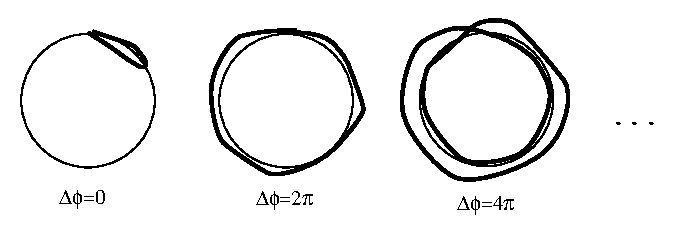
\includegraphics[scale=1.0]{pics/homotopija.eps}}
\end{primjer}
Na ovom skupu klasa krivulja može se prirodno
definirati zbrajanje. Kao reprezentante klasa uzmimo
krivulje koje počnu i završe u nekoj konkretnoj \emph{baznoj} točki, recimo $\phi=0$.
Uzmemo li dvije zatvorene krivulje, njihov zbroj definiramo kao krivulju koja se dobije tako da 
prvo po jednoj krivulji idemo od bazne točke do bazne točke, pa onda
"bez završavanja" nastavimo tako po drugoj i završimo u baznoj točki.
Obzirom na takvo zbrajanje (klasa) krivulja, ovaj skup čini grupu
poznatu pod imenom \emph{fundamentalna grupa} ili \emph{prva grupa homotopija} $\pi_1$. 
Ta grupa je temeljno topološko obilježje svake grupe. Prema gornjem
primjeru vidimo da je $\pi_1\left(\SO{2} \right) = (\mathbb{Z}, +)$.

\begin{primjer}[\SO{3}]

U prošlom odjeljku smo vidjeli da je grupna mnogostrukost od \SO{3}
lopta s identificiranim antipodnim točkama površine.
Za promatranje
klasa krivulja kao baznu točku možemo uzeti središte lopte. Sve krivulje
koje ostaju u unutrašnjosti lopte se mogu kontinuirano deformirati jedna
u drugu pa pripadaju istoj klasi. Da bi dobili novu klasu promotrimo
krivulju koja dolazi do površine u točki $A$ i onda se nastavlja u unutrašnjost
od antipodne točke $A'$. Naglasimo da je krivulja neprekinuta zahvaljujući
identičnosti $A'=A$.
Kontinuirane deformacije ove krivulje će uvijek
zadržati svojstvo prolaska površinskom točkom (kako se $A$ miče, $A'$ se
miče tako da ostane antipodna) i krivulja se ne može deformirati u krivulje
iz prve klase koje su cijele u unutrašnjosti lopte. Dakle, dobili smo
drugu klasu. Ukoliko sad promotrimo krivulje koje prolaze dvama različitim površinskim
točkama $A$ i $B$, u nadi da ćemo možda dobiti novu klasu, vidimo da je takve
krivulje moguće deformirati do situacije da se točke stope i krivulja potpuno
ubaci u unutrašnjost lopte, kako je prikazano na slici.

\centerline{\documentclass[border=3mm]{standalone}

\usepackage{tikz}
\usetikzlibrary{decorations.markings,arrows.meta}

\begin{document}
	\begin{tikzpicture}
		\begin{scope}[decoration={
			markings,
			mark=at position 0.5 with {\arrow{Triangle[scale=0.65]}}
		}]
			\draw[thick] (-3.91,1.83) coordinate (o1) circle (1.2);
			\draw (o1) ellipse (1.18 and 0.2);
			\draw[postaction={decorate}]  plot[smooth, tension=.7] coordinates {(o1) (-3.7,1.8) (-3.49,1.86) (-3.3,2) (-3.24,2.2) (-3.3,2.41) (-3.5,2.58) (-3.7,2.6) (-3.91,2.51) (-4.05,2.3) (-4.07,2.12) (-4.03,1.95) (o1)};
			\fill (o1) circle (1.5pt);
		\end{scope}
		\begin{scope}[xshift=8cm,decoration={
			markings,
			mark=at position 0.5 with {\arrow{Triangle[scale=0.65]}}
		}]
			\draw[thick] (-3.91,1.83) coordinate (o2) circle (1.2);
			\draw  (o2) ellipse (1.18 and 0.2);
			\path (o2) --++ (45:1.2) coordinate (1) node[above right]{$A$};
			\path (o2) --++ (225:1.2) coordinate (2) node[below left]{$A'$};
			\fill (o2) circle (1.5pt);
			\draw[postaction={decorate}]  plot[smooth, tension=.7] coordinates {(2) (-4.4,1.1) (-4.1,1.33) (-4.13,1.52) (-4.63,1.57) (-4.72,1.8) (-4.52,1.9) (-4.13,1.87) (o2)};
			\draw[postaction={decorate}]  plot[smooth, tension=.7] coordinates {(o2) (-3.61,1.9) (-3.49,2.2) (-3.28,2.28) (-3.05,2.3) (-3.07,2.5) (1)};
		\end{scope}
		\begin{scope}[yshift=-3.4cm,decoration={
			markings,
			mark=at position 0.5 with {\arrow{Triangle[scale=0.65]}}
		}]
			\draw[thick] (-3.91,1.83) coordinate (o3) circle (1.2);
			\draw (o3) ellipse (1.18 and 0.2);
			\path (o3) --++ (37:1.2) coordinate (3) node[above right]{$A$};
			\path (o3) --++ (230:1.2) coordinate (4) node[below left]{$A'$};
			\path (o3) --++ (110:1.2) coordinate (5) node[above left]{$B'$};
			\path (o3) --++ (285:1.2) coordinate (6) node[below right]{$B$};
			\fill (o3) circle (1.5pt);
			\draw[postaction={decorate}]  plot[smooth, tension=.7] coordinates {(4) (-4.5,1.08) (-4.29,1.15) (-4.07,1.14) (-3.87,1.06) (-3.71,0.9) (6)};
			\draw[postaction={decorate}]  plot[smooth, tension=.7] coordinates {(5) (-4.24,2.8) (-4.02,2.61) (-3.87,2.35) (o3)};
			\draw[postaction={decorate}]  plot[smooth, tension=.7] coordinates {(o3) (-3.86,1.97) (-3.71,2.13) (-3.5,2.16) (-3.29,2.22) (-3.09,2.41) (3)};
		\end{scope}
		\begin{scope}[
			xshift=4cm,
			yshift=-3.4cm,
			decoration={
				markings,
				mark=at position 0.5 with {\arrow{Triangle[scale=0.65]}}
			}
		]
			\draw[thick] (-3.91,1.83) coordinate (o4) circle (1.2);
			\draw  (o4) ellipse (1.18 and 0.2);
			\path (o4) --++ (37:1.2) coordinate (7);
			\path (o4) --++ (40:1.2) coordinate (8) node[above right]{$B'=A$};
			\path (o4) --++ (217:1.2) coordinate (9);
			\path (o4) --++ (220:1.2) coordinate (10) node[below left]{$A'=B$};
			\fill (o4) circle (1.5pt);
			\draw[postaction={decorate}] plot[smooth, tension=.7] coordinates {(o4) (-3.64,2.08) (-3.31,2.17) (-3.1,2.4) (7)};
			\draw[postaction={decorate}] plot[smooth, tension=.7] coordinates {(8) (-3.32,2.61) (-3.72,2.71) (-4.02,2.78) (-4.16,2.49) (-4,2.2) (o4)};
			\draw  plot[smooth, tension=.7] coordinates {(10) (-4.7,1.1) (-4.8,1.2) (9)};
		\end{scope}
		\begin{scope}[
			xshift=8cm,
			yshift=-3.4cm,
			decoration={
				markings,
				mark=at position 0.5 with {\arrow{Triangle[scale=0.65]}}
			}
		]
			\draw[thick] (-3.91,1.83) coordinate (o5) circle (1.2);
			\draw  (o5) ellipse (1.18 and 0.2);
			\draw[postaction={decorate}]  plot[smooth, tension=.7] coordinates {(o5)  (-3.5,2.02)  (-3.28,2.29)  (-3.5,2.51)  (-3.88,2.46)  (-3.94,2.13)  (o5)};
			\fill (o5) circle (1.5pt);
		\end{scope}
		\node at (0,1.9) {nije u istoj klasi s};
		\draw[-{Triangle[width=18pt,length=8pt]}, line width=6pt] (-2.3,-1.5) -- (-1.4,-1.5);
		\draw[-{Triangle[width=18pt,length=8pt]}, line width=6pt] (1.69,-1.5) -- (2.59,-1.5);
	\end{tikzpicture}
\end{document}}
%\centerline{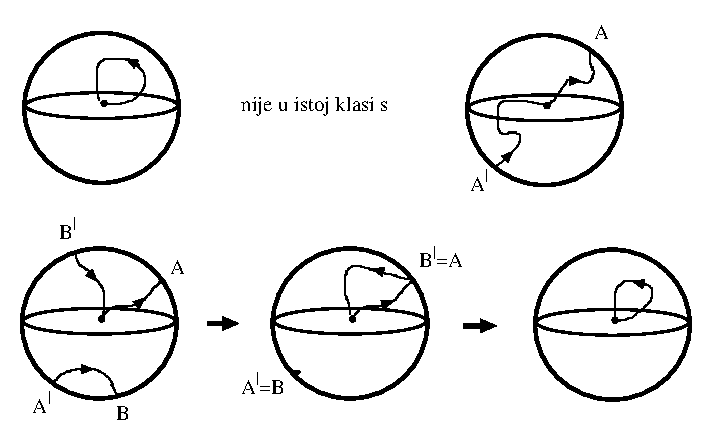
\includegraphics[scale=0.8]{pics/dvostruka_povezanost_so3.eps}}

Tako te krivulje ne čine novu nego pripadaju prvoj klasi.
Krivulja kroz tri površinske točke će se istim postupkom moći deformirati u 
krivulju kroz jednu površinsku točku i tako dalje. Dakle, postoje točno dvije klase
krivulja i kažemo da je  \SO{3} \emph{dvostruko povezana}.
Njena prva grupa homotopija je time
    $\pi_1\left(\SO{3} \right) = \mathbb{Z}_{2} = (\{+1, -1\}, \cdot)$.
\end{primjer}

\begin{primjer}[\SU{2}]
Vidjeli smo u prošlom odjeljku da je
grupna mnogostrukost \SU{2} 3-sfera tj. generalizacija uobičajene
sfere (2-sfere) na četverodimenzionalni prostor. 
Može se pokazati da je svaka $n$-sfera s $n\ge 2$ jednostavno povezana.
Pravi dokaz zahtijeva nešto znanja topologije, ali čitatelju će
moguće ta činijenica biti vrlo intuitivna, a za 2-sferu i očita.
\end{primjer}

Ako postoji homomorfizam s povezane Liejeve grupe $G$ na povezanu Liejevu
grupu $H$ s \emph{diskretnom} jezgrom $K$ onda kažemo da grupa $G$ 
\emph{pokriva} grupu $H$ onoliko puta koliko elemenata ima $K$.
(Prisjetite se teorema \ref{th:izomorfizam} o izomorfizmu.)
Također, Liejeve algebre tih grupa su izomorfne.

\begin{primjer}[\SO{3} i \SU{2}]
\SO{3} i \SU{2} su homomorfne i kako je pokazano u Dodatku \ref{sec:su2so3} 
jezgra je $\mathbb{Z}_2$. Dakle \SU{2} pokriva \SO{3} dva puta.
Kako smo vidjeli u primjeru \ref{pr:su2so3Alg}, algebre ovih
dviju grupa su izomorfne.
\end{primjer}

\begin{teorem}[Univerzalna grupa pokrivanja]
Među grupama koje pokrivaju povezanu Liejevu grupu G postoji jedinstvena
grupa koja je jednostavno povezana --- tzv. \emph{univerzalna grupa pokrivanja}.
Broj pokrivanja jednak je povezanosti od G. 
\end{teorem}


Tako je \SU{2} univerzalna grupa pokrivanja za \SO{3}.

\centerline{\documentclass[border=3mm]{standalone}

\usepackage{tikz}
\usetikzlibrary{arrows.meta}
\usepackage{amssymb}

\begin{document}
	\begin{tikzpicture}[scale=1.5]
		\node (1) at (0,0) {$\mathfrak{su}(2)$};
		\node (2) at (1.5,0) {$\mathfrak{so}(3)$};
		\node (3) at (1.5,1) {$\mathrm{SO}(3)$};;
		\node (4) at (0,1.5) {$\mathrm{SU}(2)$};
		\draw[very thick,{Triangle[scale=0.75]}-{Triangle[scale=0.75]}] (1) -- (2);
		\draw[very thick,-{Triangle[scale=0.75]}] (4.east) to[out=0,in=120,looseness=0.8] (3.north west);
		\draw[thick,-Triangle,densely dotted] (4) -- (1);
		\draw[thick,-Triangle,densely dotted] (3) -- (2);
		\draw (2,1.6) rectangle (5.7,-0.1);
		\draw[very thick,-{Triangle[scale=0.75]}] (2.1507,1.4665) to[out=0,in=120,looseness=0.8] (2.9,1.2);
		\draw[very thick,{Triangle[scale=0.75]}-{Triangle[scale=0.75]}] (2.1507,0.7839) -- (2.9,0.7839);
		\draw[thick,-Triangle,densely dotted] (2.1507,0.2881) -- (2.9,0.2881);
		\node[anchor=west] at (3.1208,1.3) {homomorfizam grupa};
		\node[anchor=west] at (3.1208,0.7839) {izomorfizam algebri};
		\node[anchor=west] at (3.1208,0.2881) {grupa $\rightarrow$ algebra};
	\end{tikzpicture}
\end{document}}
%\centerline{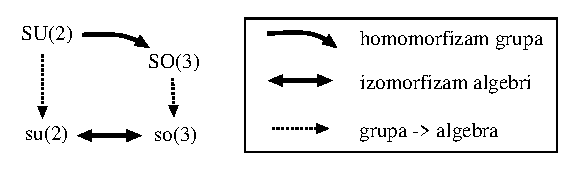
\includegraphics[scale=1.0]{pics/so3pokrivanje.eps}}

Što se grupa \SO{2} i \U{1} tiče, one su obje izomorfne i beskonačno
povezane. U primjeru \ref{pr:so2Alg} smo vidjeli da je njihova
algebra $\mathbb{R}$.
Njihovu univerzalnu grupu pokrivanja možemo identificirati
tako da identificiramo jednostavno povezanu Liejevu grupu koju
generira $\mathbb{R}$. Ako se oslonimo na eksponencijaciju
vidimo da generiramo grupu pozitivnih realnih brojeva
$\{e^{x}\,; x \in \mathbb{R}\}$ s množenjem kao grupnom operacijom.
No primjetite da je ta grupa izomorfna grupi $(\mathbb{R}, +)$
gdje je preslikavanje izomorfizma upravo eksponencijalna funkcija.
Tako možemo reći da je $R$ sam sebi algebra i sam sebi univerzalna
grupa pokrivanja, a on je i univerzalna grupa pokrivanja za
\SO{2} i \U{1}. Odgovarajući homomorfizam $\mathbb{R} \to \U{1}$
je $x \to e^{ix}$ i kernel je skup $2\pi\mathbb{Z} = \{0, \pm 2\pi,
\pm 4\pi, \ldots\}$. Riječ je o beskonačnom skupu pa kažemo da
$\mathbb{R}$ pokriva \U{1} beskonačno puta, što je konzistentno
s ranije utvrđenom činjenicom da je \U{1} beskonačno povezan.
Intuitivno je jasno da se pravac na kružnicu namata beskonačno
puta.


Općenita situacija je\\[1ex]

\centerline{\documentclass[border=3mm]{standalone}

\usepackage{tikz}
\usetikzlibrary{arrows.meta}
\usepackage{amssymb}

\begin{document}
	\begin{tikzpicture}[scale=1.5]
		\node (1) at (0,0) {$\mathfrak{ucg}$};
		\node (2) at (1.5,0) {$\mathfrak{g}_1$};
		\node (3) at (3,0) {$\mathfrak{g}_2$};
		\node (4) at (4.5,0) {$\mathfrak{g}_n$};
		\node (5) at (1.5,1) {$G_1$};
		\node (6) at (3,1) {$G_2$};
		\node (7) at (4.5,1) {$G_n$};
		\node (8) at (0,1.75) {$\mathrm{UCG}$};
		\node at (3.75,0.5) {$\cdots$};
		\draw[very thick,{Triangle[scale=0.75]}-{Triangle[scale=0.75]}] (1) -- (2);
		\draw[very thick,{Triangle[scale=0.75]}-{Triangle[scale=0.75]}] (2) -- (3);
		\draw[very thick,{Triangle[scale=0.75]}-{Triangle[scale=0.75]}] (3) -- (4);
		\draw[very thick,-{Triangle[scale=0.75]}] ([yshift=2.5pt]8.east) to[out=0,in=120,looseness=0.6] (7.north west);
		\draw[very thick,-{Triangle[scale=0.75]}] (8.east) to[out=0,in=120,looseness=0.6] (6.north west);
		\draw[very thick,-{Triangle[scale=0.75]}] ([yshift=-2.5pt]8.east) to[out=0,in=120] (5.north west);
		\draw[thick,-Triangle,densely dotted] (8) -- (1);
		\draw[thick,-Triangle,densely dotted] (5) -- (2);
		\draw[thick,-Triangle,densely dotted] (6) -- (3);
		\draw[thick,-Triangle,densely dotted] (7) -- (4);
		\node at (0.6871,1.4) {$K_1$};
		\node at (2.1,1.4) {$K_2$};
		\node at (3.6526,1.4) {$K_n$};
	\end{tikzpicture}
\end{document}}
%\centerline{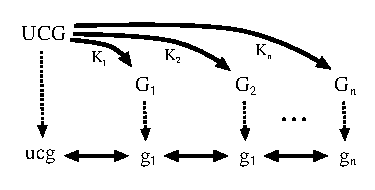
\includegraphics[scale=1.0]{pics/ucg.eps}}

gdje je UCG/$K_i$=$G_i$. Tako pronalaženjem svih diskretnih normalnih
podgrupa (kandidata za kernele homomorfizma) jednostavno povezane grupe 
možemo naći sve grupe koje
s njom dijele istu Liejevu algebru\footnote{To je znatno olakšano teoremom
koji kaže da su diskretne normalne podgrupe nužno sadržane u
centru grupe (vidi zadatak \ref{zad:centar}) što znači da svi elementi
kernela komutiraju sa cijelom grupom.}.
U zaključku, Liejeve algebre u velikoj mjeri određuju Liejevu grupu i
glavna informacija o grupi koju gubimo razmatrajući samo algebru
je njena topologija. Algebra, koja je određena okolinom jediničnog
elementa grupe "ne vidi" je li se grupa možda netrivijalno "preklapa"
na samu sebe daleko od jedinice.


\section{Klasične Liejeve grupe važne za fiziku}
\label{sec:primjeriLie}

\begin{enumerate}[leftmargin=0pt, itemindent=0pt]

\item \textbf{Opća linearna grupa}

Opću linearnu grupu $\GL{n, \mathbb{C}}$ čini
skup svih $n\times n$ regularnih ($\det M \neq 0$)
kompleksnih matrica
Kako je svaka matrica zadana s $n^2$ nezavisnih kompleksnih brojeva, ova
grupa ima $2 n^2$ realnih parametara. Uvjet regularnosti nije ograničenje
koje smanjuje broj parametara, jer je samo riječ o zahtjevu da determinanta,
koja je izraz koji uključuje tih $2 n^2$ parametara bude \emph{različita} od nule.

\begin{equation}
\det M = f(a_1, a_2 , \dots, a_{2n}) \neq 0
\end{equation}

Podgrupa ove grupe je grupa $\GL{n, \mathbb{R}}$ koja očito ima samo
$n^2$ parametara. $\GL{n, \mathbb{R}}$ ima dvije komponente povezanosti,
jednu čine matrice pozitivne, a drugu matrice negativne komponente.
Izuzeće determinante nula razdvaja te komponente, ali to nije slučaj
za $\GL{n, \mathbb{C}}$ koja je povezana (ali ne i jednostavno povezana).

\item \textbf{Specijalna linearna grupa}

\begin{equation}
\SL{n, \mathbb{C}} = \{ M\in \GL{n,\mathbb{C}} \; | \; \det M = 1\}
\end{equation}

Ovdje je na svaku matricu postavljen dodatni uvjet
\begin{equation}
\det M = f(a_1, a_2 , \dots, a_{2n}) = 1 \;,
\label{eq:SL}
\end{equation}
koji predstavlja jednu kompleksnu, tj. dvije realne jednadžbe koje
se mogu iskoristiti za eliminaciju dvaju parametera. Tako ova grupa
ima $2 n^2 - 2$ parametara. Grupa je jednostavno povezana i za fiziku
je posebno važna grupa $\SL{2, \mathbb{C}}$ koja je univerzalna grupa
pokrivanja za Lorentzovu grupu na analogan način na koji je \SU{2}
univerzalna grupa pokrivanja za grupu rotacija \SO{3}.

Podgrupa ove grupe je grupa $\SL{n, \mathbb{R}}$ koja ima 
$n^2 - 1$ parametar. (Jednadžba (\ref{eq:SL}) je sad samo jedna
realna jednadžba, a ne dvije.) Ona je povezana, ali ne i jednostavno
povezana.

\item \textbf{Unitarna grupa}

\begin{equation}
\U{n} = \{ M\in \GL{n,\mathbb{C}} \; | \; M M^{\dagger} = 1\}
\end{equation}
Prebrojavanje nezavisnih parametara za ovu grupu može se izvesti
na više načina. Uvjet $M M^\dagger = 1$ se može napisati izraženo
preko komponenti matrica kao (u ovom odjeljku ćemo radi jasnoće
suspregnuti Einsteinovu sumacijsku konvenciju i pisati sume eksplicitno)
\begin{equation}
\sum_{j=1}^{n} M_{ij} M_{kj}^* = \delta_{ik}\;,
\label{eq:unitaritycondition}
\end{equation}
gdje je iskorišteno $M^{\dagger}_{jk} = M^{*}_{kj}$.
Jednadžba (\ref{eq:unitaritycondition}) predstavlja $n^2$ kompleksnih
jednadžbi ali sve one nisu nezavisne. Promotrimo prvo $n$ jednadžbi
određenih uvjetom $i=k$ (dakle gledamo dijagonalu te matrične jednadžbe):
\begin{equation}
 \sum_j M_{ij} M^{*}_{ij} = \sum_j |M_{ij}|^2 = 1 \,.
\label{eq:diagonalcondition}
\end{equation}
To je $n$ realnih jednadžbi koje se mogu upotrijebiti za eliminiranje
$n$ parametara. Dalje možemo gledati jednadžbe određene uvjetom
$i < k$ (dakle gledamo trokut iznad dijagonale matrične jednadžbe).
Te su jednadžbe kompleksne i ima ih $n(n-1)/2$ (broj elemenata u 
spomenutom trokutu). Sve ove jednadžbe su neovisne pa se mogu
iskoristiti za eliminiranje $2 \cdot n(n-1)/2 = n(n-1)$ parametara.
Preostaju jednadžbe za $i >k$ (donji trokut matrice), ali kompleksnom
konjugacijom odgovarajućih jednadžbi
\begin{equation}
\sum_{j=1}^{n} M_{ij} M_{kj}^* = 0\,, \qquad i>k \,,
\end{equation}
dobijemo
\begin{equation}
\sum_{j=1}^{n} M_{ij}^* M_{kj}  = \sum_{j=1}^{n} = M_{kj} M_{ij}^* = 0\,, \qquad i>k \,,
\end{equation}
pa uz preimenovanje indeksa $i \leftrightarrow k$
\begin{equation}
\sum_{j=1}^{n} =  M_{ij} M_{kj}^* = 0\,, \qquad k>i \,,
\end{equation}
vidimo da su ove jednadžbe ekvivalentne ovima iz gornjeg trokuta tj. nisu
nezavisne.
Znači sve skupa možemo eliminirati $n + n(n-1) = n^2$ parametara, pa ih
ostane $2n^2 - n^2 = n^2$ što je broj parametara unitarne grupe.
(Drugi način prebrojavanja je da se iskoristi da su retci matrice ortonormirani
vektori. Uvjet normalizacije daje $n$ realnih jednadžbi, a uvjet
ortonogonalnosti $\binom{n}{2}$ kompleksnih, gdje se treba uvjeriti
da odgovarajući zahtjevi na stupce nisu nezavisni od ovih na retke.)
Unitarna grupa je kompaktna i povezana, ali ne i jednostavno. Za $\U{1}$
smo vidjeli, a i za ostale unitarne grupe
vrijedi da im je prva grupa homotopije $\pi_{1}(\U{n}) = \mathbb{Z}$.

Važno svojstvo unitarnih matrica je da, ukoliko ih interpretiramo kao
operatore nad kompleksnim vektorskim prostorima ($\vec{x} \to M\vec{x}$), 
one čuvaju skalarni produkt
\begin{align}
    (\vec{x}, \vec{y})& = \sum_{i=1}^n x_{i}^* y_i  \longrightarrow
   \sum_{ijk} M^{*}_{ij}x^{*}_j M_{ik}y_{k} \nonumber \\
 & = \text{uvrštavanjem
 (\ref{eq:unitaritycondition})} = \sum_{kj} \delta_{kj} x^{*}_j y_k = (\vec{x}, \vec{y})
\label{eq:productinvariance}
\end{align}
Lako je pokazati da se ovo može uzeti kao alternativna definicija
unitarne grupe tj. da se unitarne matrice mogu definirati kao one koje
čuvaju ovaj skalarni produkt, a onda je svojstvo $M^{\dagger} M = 1$, koje
smo ovdje uzeli kao definiciono, samo posljedica.

\item \textbf{Specijalna unitarna grupa}

\begin{equation}
\SU{n} = \{ M\in U(n) \; | \; \det M  = 1\}
\end{equation}

Za prebrojavanje parametara treba prvo uočiti da je za sve unitarne
matrice determinanta ograničena na apsolutnu vrijednost 1. To slijedi
primjenom Binet-Cauchyjevog teorema na definiciju $M M^{\dagger} = 1$
što daje $|\det M|^2 = 1$ odnostno $\det M = e^{i \phi}$, 
$\phi\in [0, 2\pi)$.
Dodatni uvjet za specijalne unitarne matrice $\det M = 1$ je onda
samo jedna realna jednadžba $\phi = 0$ pa specijalna unitarna grupa
ima točno $n^2 - 1$ parametar. \SU{n} su kompaktne i jednostavno povezane.

\item \textbf{Ortogonalna grupa}

\begin{equation}
\O{n, \mathbb{C}} = \{ M\in \GL{n,\mathbb{C}} \; | \; M M^{\mathrm{T}} = 1\}
\end{equation}

Kod prebrojavanja parametara, jedina razlika obzirom na unitarne matrice
je da umjesto ($i=k$) jednadžbi (\ref{eq:diagonalcondition}) 
koje odgovaraju dijagonali matrične jednadžbe sada imamo
\begin{equation}
 \sum_j M_{ij} M_{ij} = \sum_j M_{ij}^2 = 1
\end{equation}
što su kompleksne jednadžbe pa možemo eliminirati sve skupa
$2n + n(n-1)$ parametara i ostaje ih samo $n(n-1)$.

U fizici se najčešće susrećemo s grupom ortogonalnih \emph{realnih} matrica
\begin{equation}
\O{n} \equiv \O{n, \mathbb{R}} = \{ M\in \GL{n,\mathbb{R}} \; | \; M M^{\mathrm{T}} = 1\}
\end{equation}
koja ima $n(n-1)/2$ parametara. Ova grupa čuva
kvadratnu formu $(\vec{x}, \vec{y}) = \sum_i x_i y_i$ tj. skalarni produkt na realnom
vektorskom prostoru, što se može upotrijebiti kao alternativna definicija grupe.

\item \textbf{Specijalna ortogonalna grupa}

\begin{equation}
\SO{n, \mathbb{C}} = \{ M\in O(n, \mathbb{C}) \; | \; \det M  = 1\} \;,
\end{equation}
i odgovarajuća realna grupa $\SO{n}$ imaju isti broj parametara kao
$\O{n, \mathbb{C}}$, odnosno \O{n}. Naime, uvjet ortogonalnosti
$M M^{\mathrm{T}} = 1$ vodi na $(\det M)^2 = 1$, odnosno
na zaključak da ortogonalne matrice imaju determinantu $\det M = \pm 1$,
pa ograničenje na $\det M = 1$ ne smanjuje dimenziju parametarskog prostora.

\item \textbf{Pseudo-unitarna grupa}

Čine je $n\times n$ matrice
\begin{equation}
\U{p, q} = \{ M\in \GL{n,\mathbb{C}} \; | \; M^{\dagger} g M = g\} \;,
\end{equation}
gdje je $p+q=n$ i gdje je $g$ dijagonalna matrica oblika
\begin{equation}
  g = \mathrm{diag}(\underbrace{1, 1, \dots, 1}_{p \times},
\underbrace{-1, -1, \dots, -1}_{q \times}) \;.
\label{eq:metricg}
\end{equation}
Ova grupa ima isti broj parametara kao i $\U{n}$, te
čuva kvadratnu formu oblika
\begin{equation}
 \sum_{i=1}^{p} x_{i}^* y_{i} - \sum_{i=p+1}^{p+q=n} x_{i}^* y_i 
\end{equation}
koja nije pozitivno definitna pa nije skalarni produkt u smislu
definicije \ref{def:skalarniprodukt}.


\item \textbf{Pseudo-ortogonalna grupa}

\begin{equation}
\O{p, q} = \{ M\in \GL{n,\mathbb{R}} \; | \; M^{\mathrm{T}} g M = g \} \;,
\label{eq:MgM}
\end{equation}
gdje je $p+q=n$ i gdje je $g$ dijagonalna matrica iz (\ref{eq:metricg}).
Ove matrice čuvaju kvadratnu formu oblika
\begin{equation}
 \sum_{i=1}^{p} x_{i} y_{i} - \sum_{i=p+1}^{p+q=n} x_{i} y_i  \;.
\end{equation}
Najpoznatija grupa ove vrste je grupa Lorentzovih transformacija  $\O{1,3}$
(vidi odjeljak \ref{sec:lorentz}). Ove grupe su nekompaktne i imaju
četiri komponente povezanosti što za 
konkretan primjer grupe $O(1,3)$ pokazujemo u odjeljku \ref{sec:lorentz}.

Specijalnu pseudo-unitarnu grupu $\SU{p,q}$ odnosno specijalnu
pseudo-or\-to\-go\-nal\-nu
grupu $\SO{p,q}$ dobivamo ako se u $\U{p,q}$ odnosno $\O{p, q}$
ograničimo na matrice s $\det M = 1$.

\end{enumerate}


U preostalim poglavljima knjige bavit ćemo se sa samo nekoliko grupa
koje su se pokazale od najveće važnosti za primjene u fizici, no recimo
ipak nešto o kompletnom katalogu Liejevih grupa.

Kao prvo, mi smo ovdje, kao i mnogi autori, posebice fizičari, razlikovali
Liejeve (kontinuirane) grupe i diskretne grupe. To je na ovom nivou pedagoški
poželjno kako bi se istaknula specifična moć netrivijalnih Liejevih algebri tj. infinitezimalne
okoline jedinice. No, strogo uzevši, i skup diskretnih točaka je
(0-dimenzionalna) mnogostrukost, a i topološki prostor (s tzv. 
diskretnom topologijom, vidi \cite{Smolic:2024}) tako da su i diskretne
i konačne grupe zapravo strogo uzevši Liejeve, što nas onda spašava od
nezgodnih situacija da formiranjem kvocijentnih skupova ne izlazimo
iz domene Liejevih grupa.

Kad je to rečeno, recimo da su kontinuirane kompaktne Liejeve grupe
lakše za potpunu klasifikaciju. Kao prvo,
bitno je klasificirati jednostavne grupe, jer ukoliko grupa ima normalne
podgrupe onda se može reducirati uzimanjem kvocijenta po toj podgrupi
(jednostavne grupe su poput prostih brojeva teorije grupa). W. Killing i \'{E}. Cartan
su pokazali da algebre tih grupa spadaju u jednu od četiri beskonačne 
porodice u matematici poznate kao $\mathrm{A}_n, \mathrm{B}_n, \mathrm{C}_n$
i $\mathrm{D}_n$, gdje već poznajemo
$\mathrm{A}_n$ kao algebre od $\SU{n+1}$,  $\mathrm{B}_n$ kao algebre od \SO{2n+1},
$\mathrm{D}_n$ kao algebre od \SO{2n}, a $\mathrm{C}_n$ su algebre tzv. simplektičkih grupa
$\mathrm{Sp}(n)$ koje isto imaju neke primjene u fizici, ali mi ih ovdje
nećemo više spominjati. Osim ove četiri porodice postoji još samo
pet \emph{iznimnih} grupa $\mathrm{G}_2$, $\mathrm{F}_4$,
$\mathrm{E}_6$, $\mathrm{E}_7$, i $\mathrm{E}_8$ koje nalaze svoju primjenu
u nekim teorijama unifikacije sila u prirodi i teoriji superstruna.

Kod diskretnih jednostavnih grupa imamo kao prvo cikličke grupe $\mathrm{C}_{p}$
gdje je $p$ prost broj i koje smo upoznali, 
zatim alternirajuće grupe $\mathrm{A}_{n\ge 5}$ parnih permutacija skupova
od $n$ elemenata (pomoću kojih je Galois pokazao nerješivost jednadžbi
reda većeg od pet) i
veliku porodicu diskretnih grupa tzv. Liejevog tipa koje su konstruirane
kao standardne Liejeve grupe, ali ne nad poljem realnih brojeva nego
nad konačnim poljima. Povrh toga postoji još samo 26 tzv. \emph{sporadičnih}
grupa\footnote{Četiri sporadične grupe je pronašao hrvatski matematičar Zvonimir Janko
i po njemu se zovu $\mathrm{J}_{1, 2, 3, 4}$.} gdje je najveća od njih
čuvena grupa \emph{čudovište} (engl. \emph{monster}) s
\[ \textstyle
808\,017\,424\,794\,512\,875\,886\,459\,904\,961\,710\,757\,005\,754\,368\,000\,000\,000
\]
odnosno približno $8\times 10^{53}$ elemenata. Njena primjena u fizici je samo u domeni spekulacija, no
neke ideje iz fizike su iskorištene za određivanje svojstava te komplicirane
grupe.




\subsection*{Zadaci za vježbe}

\begin{enumerate}[label=\arabic{chapter}.\arabic*.]

\item \label{zad:O3oSO3} Uvjerite se da je kvocijentna grupa $\O{3}/\SO{3} = \mathrm{C}_{2}$.

\item \label{zad:svojstvalevicivite} Pokažite da Levi-Civita tenzor ima slijedeća svojstva:
\begin{align*}
\tag{a}\epsilon_{ijk}\epsilon_{imn}&=\delta_{jm}\delta_{kn}-\delta_{jn}\delta_{km}\\
\tag{b}\epsilon_{ijk}\epsilon_{ijm}&=2\delta_{km} \\
\tag{c}\epsilon_{ijk}\epsilon_{ijk}&=6 \\
\tag{d}\epsilon_{ijk}a_j b_k &= (\vec{a}\times\vec{b})_i  \\
\tag{e}\frac{1}{3!}\epsilon_{lmn} \epsilon_{ijs} A_{li} A_{mj} A_{ns} &= \det A
\end{align*}

\item Uporabom svojstava Levi-Civita tenzora pokažite da je
za vektore $\vec{a}$, $\vec{b}$ i \vec{c}
\begin{displaymath}
    \vec{a}\times(\vec{b}\times\vec{c})=(\vec{a}\cdot\vec{c})\vec{b}
 -(\vec{a}\cdot\vec{b})\vec{c}
\end{displaymath}
\secret{Za slične stvari vidi Evett, Am. J. Phys \textbf{34} (1966) 503.}

\item \label{zad:svojstvapaulijevih} Pokažite da Paulijeve matrice imaju slijedeća svojstva:
\begin{align*}
\tag{a} \sigma_{i}^2 &= 1 \\
\tag{b} \sigma_{i}^\dagger &= \sigma_i \\
\tag{c} \det \sigma_i &= -1 \\
\tag{d} \Tr \sigma_i &=0 \\
\tag{e} [\sigma_i, \sigma_j] &= 2 i \epsilon_{ijk} \sigma_k \\
\tag{f} \{\sigma_i, \sigma_j\}\equiv \sigma_i\sigma_j + \sigma_j \sigma_i &= 2
\delta_{ij} 1 \\
\tag{g} \Tr (\sigma_i \sigma_j) &= 2\delta_{ij} \\
\tag{h} \sigma_i \sigma_j &= \delta_{ij} 1 + i \epsilon_{ijk}\sigma_k\\
\tag{i} e^{-\frac{i}{2}\vec{\sigma}\cdot\unitn \theta} &=
\cos \frac{\theta}{2}-i\vec{\sigma}\cdot\unitn \sin\frac{\theta}{2} \quad\in \SU{2}
\end{align*}

\item \label{zad:abelovaalgebra} Za Abelovu grupu vrijedi $g_1 g_2 g_{1}^{-1} g_{2}^{-1} = e$,
    gdje se $g_1 g_2 g_{1}^{-1} g_{2}^{-1}$ naziva \emph{komutator} elemenata grupe.
    Ako je $g_1$ generiran elementom algebre $g_1 = e^{s X}$, a $g_2 = e^{t Y}$, gdje su
    $s$ i $t$ realni parametri, pokažite da je
\begin{equation}
\frac{\partial^2}{\partial s \, \partial t} \bigg|_{s=t=0} \big( \exp(sX) \exp(tY)
\exp(-sX) \exp(-tY) \big) = [X, Y] \,,
\end{equation}
i time da je algebra $\calA$ Abelove grupe trivijalna $[X, Y] = 0$, za svake $X, Y \in \calA$.

\item Provjerite eksplicitno BCH formulu do kubičnog člana.


\item Pokažite da matrice
\begin{equation}
 M(\theta) = \begin{pmatrix}
\cosh\theta & \sinh\theta  \\
\sinh\theta & \cosh\theta
\end{pmatrix}
\end{equation}
djelujući na vektore $(x, y)$ čuvaju formu $x^2 - y^2$, te da 
je $\det M(\theta) = 1$, tako da $M(\theta)$ tvore grupu
$\SO{1,1}$.
\item Grupni prostor kvocijentne grupe $G/H$ Liejeve grupe $G$ po diskretnoj normalnoj podgrupi $H$
    općenito odgovara grupnom prostoru od $G$ u kojem su su sve točke svake susjedne klase po $H$
    identificirane. Tako je grupni prostor $\SU{2}/\mathbb{Z}_2$ 3-sfera s identificiranim
    antipodnim točakama $S^{3}/\mathbb{Z}_2$. 
    No kako je $\SU{2}/\mathbb{Z}_2 = \SO{3}$, a grupni prostor od
    \SO{3} je puna 3D \emph{lopta} s identificiranim nasuprotnim točkama, $B^{3}/\mathbb{Z}_2$,
    slijedi da su ta dva prostora topološki jednaka tj. jedan te isti prostor,
    $B^{3}/\mathbb{Z}_2 = S^{3}/\mathbb{Z}_2$.
    Uvjerite se da je to zaista tako, promatrajući
    preslikavanje s $B^{3}$ na $\mathbb{R}^4$ dano s
    \begin{multline}
        f(r, \theta, \phi) = \\ \left( 
            \cos\left(\frac{r}{2}\right), 
            \sin\left(\frac{r}{2}\right)\cos\theta, 
            \sin\left(\frac{r}{2}\right)\sin\theta\cos\phi, 
            \sin\left(\frac{r}{2}\right)\sin\theta\sin\phi 
            \right) \,.
    \end{multline}
    Inače, navedeni prostor matematičari zovu \emph{realni projektivni prostor}
    $\mathbb{RP}^{3}$.
\end{enumerate}
